% Copyright 2004 by Till Tantau <tantau@users.sourceforge.net>.
%
% In principle, this file can be redistributed and/or modified under
% the terms of the GNU Public License, version 2.
%
% However, this file is supposed to be a template to be modified
% for your own needs. For this reason, if you use this file as a
% template and not specifically distribute it as part of a another
% package/program, I grant the extra permission to freely copy and
% modify this file as you see fit and even to delete this copyright
% notice. 

% \UseRawInputEncoding
\documentclass{beamer}

% There are many different themes available for Beamer. A comprehensive
% list with examples is given here:
% http://deic.uab.es/~iblanes/beamer_gallery/index_by_theme.html
% You can uncomment the themes below if you would like to use a different
% one:
%\usetheme{AnnArbor}
%\usetheme{Antibes}
%\usetheme{Bergen}
%\usetheme{Berkeley}
%\usetheme{Berlin}
%\usetheme{Boadilla}
%\usetheme{boxes}
%\usetheme{CambridgeUS}
%\usetheme{Copenhagen}
%\usetheme{Darmstadt}
%\usetheme{default}
%\usetheme{Frankfurt}
%\usetheme{Goettingen}
%\usetheme{Hannover}
%\usetheme{Ilmenau}
%\usetheme{JuanLesPins}
%\usetheme{Luebeck}
\usetheme{Madrid}
%\usetheme{Malmoe}
%\usetheme{Marburg}
%\usetheme{Montpellier}
%\usetheme{PaloAlto}
%\usetheme{Pittsburgh}
%\usetheme{Rochester}
%\usetheme{Singapore}
%\usetheme{Szeged}
%\usetheme{Warsaw}

\usepackage{pgfgantt}
\usepackage{todonotes}
\usepackage{media9}
% \usepackage{subfigure}
\usepackage{booktabs,array}
\usepackage[font=tiny,labelfont=bf]{caption}
\usepackage{tabulary}
\usepackage{caption}
\usepackage{graphicx}
\usepackage{siunitx}
\usepackage{arydshln}
\usepackage{rotating}
\usepackage{amsmath,amssymb,amsfonts,bm}
\usepackage{tikz}


% Customize Warsaw color 
\setbeamercolor*{palette primary}{use=structure,fg=white,bg=red!50!black}
\setbeamercolor*{palette secondary}{use=structure,fg=white,bg=red!60!black}
\setbeamercolor*{palette tertiary}{use=structure,fg=white,bg=red!70!black}

% Customize Warsaw block title and background colors
\setbeamercolor{block title}{bg=red!50!black,fg=white}

\setbeamertemplate{navigation symbols}{} % Remove navigation symbols
\setbeamertemplate{bibliography item}{\insertbiblabel}  % insert bibliography numbers instead of symbol
\setbeamertemplate{caption}[numbered] % adds the figure or table number to the caption.

% Set up footer manually
\setbeamertemplate{footline}
{
  \leavevmode%
  \hbox{%
  \begin{beamercolorbox}[wd=.45\paperwidth,ht=2.25ex,dp=1ex,center]{author in head/foot}%
    \usebeamerfont{author in head/foot}\insertshortauthor\hspace*{1em}(\insertshortinstitute)
  \end{beamercolorbox}%
  \begin{beamercolorbox}[wd=.4\paperwidth,ht=2.25ex,dp=1ex,center]{title in head/foot}%
    \usebeamerfont{title in head/foot}\insertshorttitle
  \end{beamercolorbox}%
  \begin{beamercolorbox}[wd=.15\paperwidth,ht=2.25ex,dp=1ex,center]{date in head/foot}%
    \usebeamerfont{date in head/foot}\insertframenumber{} / \inserttotalframenumber
  \end{beamercolorbox}}%
  \vskip0pt%
}

%==============================================================================
%     TITLE
%==============================================================================
\title[HIL Plant Modeling]{Data-Driven Hardware-in-the-Loop Plant Modeling for Self-Driving Vehicles}

\author[H.~Grady, N.~Nauman, Md Suruz~Miah]{Hannah~Grady \and Nicholas~Nauman \and Md Suruz~Miah}
% - Give the names in the same order as the appear in the paper.
% - Use the \inst{?} command only if the authors have different
%   affiliation.

\institute[Bradley University] % (optional, but mostly needed)
{
  \inst{~}Department of Electrical and Computer Engineering\\
  Bradley University, Peoria, Illinois, 61625, USA
  \and
  \inst{~}\textbf{Sponsor:}~AutonomouStuff $|$~https://autonomoustuff.com/\\
  306 Erie Avenue, Morton, IL 61550\\
  Telephone:~309-291-0966, email:info.as.ap@hexagon.com
}
% - Use the \inst command only if there are several affiliations.
% - Keep it simple, no one is interested in your street address.
%



\date[IEEE ROSE,~2022]{IEEE International Symposium on Robotics and Sensors Environments $|$ Nov. 14-15,~2022 $|$ Hybrid $|$ Khalifa University, Abu Dhabi UAE}

% - Either use conference name or its abbreviation.
% - Not really informative to the audience, more for people (including
%   yourself) who are reading the slides online

\logo{\hfill\href{http://www.bradley.edu}{
\includegraphics[width=0.75cm]{figs/logoBU1-Print}}}  % place logo in every page 


\subject{Plant Modeling for Autonomous Vehicle}
% This is only inserted into the PDF information catalog. Can be left
% out. 

% If you have a file called "university-logo-filename.xxx", where xxx
% is a graphic format that can be processed by latex or pdflatex,
% resp., then you can add a logo as follows:

% \pgfdeclareimage[height=0.5cm]{university-logo}{university-logo-filename}
% \logo{\pgfuseimage{university-logo}}

% Delete this, if you do not want the table of contents to pop up at
% the beginning of each subsection:
\AtBeginSection[]
{
  \begin{frame}<beamer>{Outline}
    \tableofcontents[currentsection,currentsubsection]
  \end{frame}
}

%==============================================================================
%==============================================================================
%     START OF SLIDES
%==============================================================================
%==============================================================================

% Let's get started
\begin{document}

\begin{frame}
  \titlepage
\end{frame}

\begin{frame}{Outline} 
  \tableofcontents%[pausesections]
  % You might wish to add the option [pausesections]
\end{frame}

% Section and subsections will appear in the presentation overview
% and table of contents.
\section{Introduction}

\begin{frame}{Introduction}{}
	\begin{block}{Applications of Autonomous Vehicles}
    	\begin{itemize}
    		\item Autonomous vehicles are being developed by many companies for commercial and personal use
    		\item Modeling different subsystems (such as, steering, brake,
          acceleration, $\ldots$)  for autonomous vehicles is a challenging task
     		\item Models for autonomous vehicle subsystems must be very accurate due to safety factors
		\end{itemize}
    \end{block}
        \begin{figure}
			\centering
			\begin{minipage}[t]{0.4\textwidth}
				\centering
				\includegraphics[height=1.5cm]{figs/img/autonomousVehiclesAStuff}
				\caption{AutonomouStuff Vehicle Fleet\textsuperscript{a}}
				\label{fig:fleet}
			\end{minipage}
			\begin{minipage}[t]{0.4\textwidth}
				\centering
				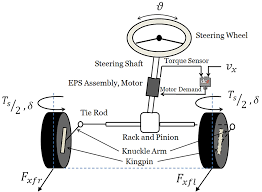
\includegraphics[height=1.5cm]{figs/img/autonomousVehiclesSteering}
				\caption{Autonomous Vehicle Steering System\textsuperscript{b}}
				\label{fig:steerSystem}
			\end{minipage}
        \end{figure}
    \begin{tiny}
		\textsuperscript{a}https://hexagonpositioning.com/pi-brands/autonomoustuff\\\textsuperscript{b}https://www.autonews.com/article/20181105/OEM10/181109921/delphi-s-pace-award-winning-e-steer-an-autonomous-vehicle-building-block
    \end{tiny}
\end{frame}



\begin{frame}{Introduction}{Problem Statement}
  \begin{block}{Problem Statement}
    Given input-output data of different subsystems, such as steering, acceleration, brake, shift, speed, and speed control, of an autonomous (self-driving) vehicle:
    \begin{itemize}
    \item Develop mathematical and/or block diagram models of these subsystems 
      
    \item Develop machine learning-based models for the major subsystems of Lexus self-driving vehicle
    \end{itemize}
  \end{block}
  \pause
  \begin{block}{Proposed Solution}
    \begin{itemize}
    \item Use state-space modeling techniques based on input and output data 
     
    \item Use system identification modeling techniques
      
    \item Use machine learning (neural network) based modeling techniques
    \end{itemize}
  \end{block}
\end{frame}

%----------------------------------

%----------------------------------
\section{Literature Review}

\begin{frame}{Literature Review}{}
	\begin{block}{Existing Solutions}
 	\begin{itemize}
        \item Use of System Identification Toolbox in MATLAB to create models from data~\cite{Adnan2010}
	 \begin{itemize}
     \tiny
		    		\item Offers a variety of model choices
				\item Needs a large amount of raw data to produce an accurate model
	\end{itemize}
	\item Third order ARMAX model creates models using traditional methods of analysis~\cite{Li1999}
	 \begin{itemize}
     \tiny
		    		\item Allows the use of traditional analysis methods to create a model 
				\item More room for error during calculations
	\end{itemize}
	\item Steer-By-Wire method as a system model~\cite{Saruchi2015}
	 \begin{itemize}
     \tiny
		    		\item Can model systems with small non-linearities 
				\item Mechanical components replaced by electrical components 
	\end{itemize}
	\item Authors in~\cite{Hussain2011} illustrate identification of multiple-input single-output model for maximum power point tracking of photovoltaic system.  
	\begin{itemize}
    \tiny
		\item Fourth order ARX model ended up giving the best fit
	\end{itemize}
\end{itemize}
  \end{block}
\end{frame}

%---------------------------
\section{System Identification Preliminaries}

\begin{frame}{System Identification Preliminaries}{}
  \begin{block}{Preliminary Work}
 \begin{itemize}
        \item Documentation on MATLAB's System Identification Toolbox and tutorials
        \item Literature Review 
        \item Data Collection for steering, braking and acceleration subsystems
\end{itemize}
  \end{block}
  
   \begin {block}{MATLAB Example: Dealing with Multi-Variable Systems: Identification and Analysis}
  \begin{itemize}
  	\item  Learned how to create an iddata object from a given data set 
  	\item Created a state space model and compared it to the validation data 
  	\item Tried creating submodels for some of the channels in order to try and get a better fit 
  	\item Then created a MISO model and learned how to merge the two SISO models that were created earlier 
  	\end{itemize}
  	\end{block}
\end{frame}

%-------------------------
\section{System Architecture}

\begin{frame}{System Architecture}{}
%  \missingfigure{Place the overall vehicle picture from the report that shows different subsystems  }
\begin{figure}
				\centering
				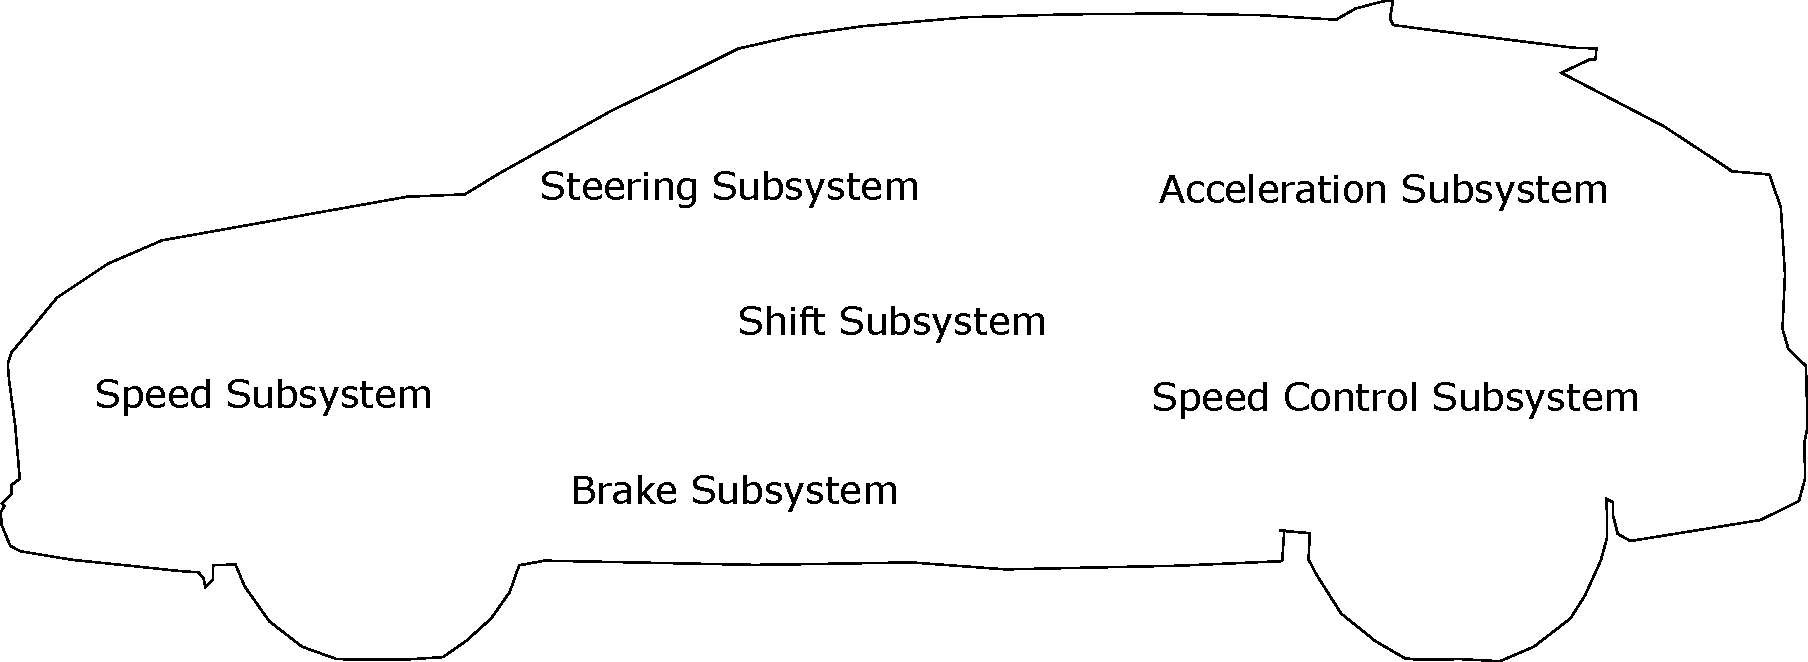
\includegraphics[height=3.5cm]{figs/inkscape/carSystemModelOutline}
				\label{fig:carSystemSubsystem}
				\caption{Lexus Vehicle with Subsystems}
        \end{figure}
%	\begin{block}{System Architecture}
%    The overall system architecture of this project consists of six subsystems: 
%    \begin{itemize}
%        \item Steering
%        \item Acceleration
%        \item Brake %Model
%        \item Shift %Model
%        \item Speed %Model
%        \item Speed control %Model
%      \end{itemize} 
%  \end{block}
\end{frame}

\begin{frame}{System Architecture}{}
	\begin{block}{System Architecture}
    The overall system architecture of this project consists of six subsystems: 
    \begin{itemize}
        \item Steering
        \item Acceleration
        \item Brake %Model
        \item Shift %Model
        \item Speed %Model
        \item Speed control %Model
      \end{itemize} 
  \end{block}
\end{frame}

\begin{frame}{System Architecture}{Subsystems}

\begin{figure}
  \centering
  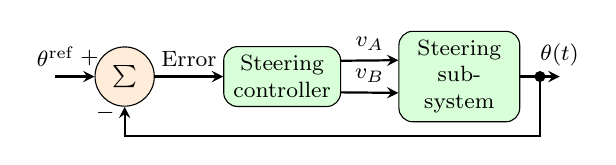
\begin{tikzpicture}
    \tikzstyle{every node} = [font=\footnotesize]
    \tikzstyle{block} = [draw, rectangle, fill=green!15, rounded corners=5pt, minimum width=1 cm, minimum height=0.75 cm]
    \tikzstyle{sum} = [draw, circle,fill=orange!15]
    % place nodes
    \node[sum](sum){$\sum$};
    \node[block,right of=sum,node distance=2 cm, text width=1.25cm,text centered](steeringController){Steering controller};
    \node[block,right of=steeringController,node distance=2.25 cm, text width=1.3cm,text centered](steeringSubsystem){Steering subsystem};

    % Connections
    \draw[stealth-,thick]
    (sum.west)--node[very near start,above]{$+$}++(-0.5,0)node[above]{$\theta^{\text{ref}}$};
    \draw[-stealth,thick]
    (sum.east)--node[midway,above]{Error}(steeringController);
    \draw[-stealth,thick]
    (steeringController.15)--node[midway,above]{$v_A$}(steeringSubsystem.165);
    \draw[-stealth,thick]
    (steeringController.-15)--node[midway,above]{$v_B$}(steeringSubsystem.-165);
    \draw[-stealth,thick]
    (steeringSubsystem.east) --coordinate (tt) ++(0.5,0)node[above]{$\theta(t)$};
    \fill
    ($(steeringSubsystem.east)+(0.25,0)$) circle [radius=2pt];
    \draw[-stealth,thick]
    (tt) -- ++(0,-0.75) -|(sum.south)node[pos=0.9,left]{$-$};
    
  \end{tikzpicture}
  % \captionsetup{justification=centering, margin=3cm}

  % 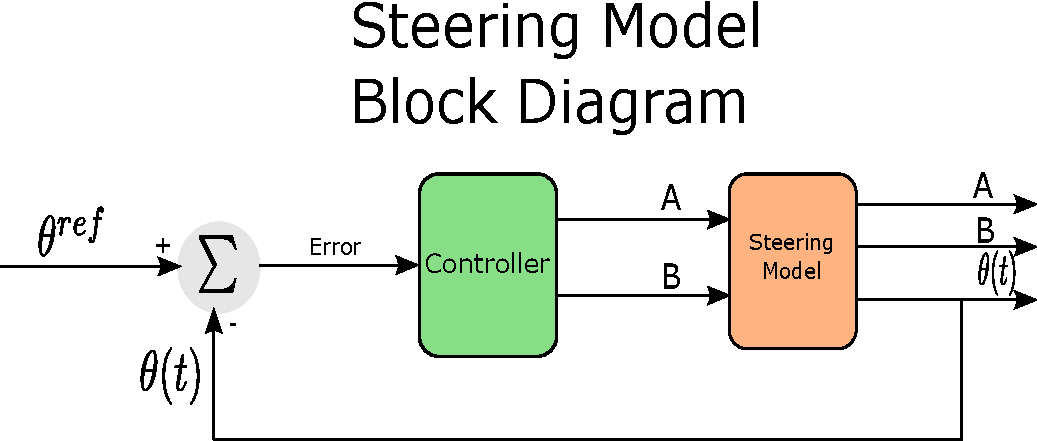
\includegraphics[width=2.5in]{figs/inkscape/steeringModelBlockDiagram}
  \caption{Steering subsystem block diagram.}
  \label{fig:steeringModelBlockDiagram}
\end{figure}


\begin{figure}
    \centering
  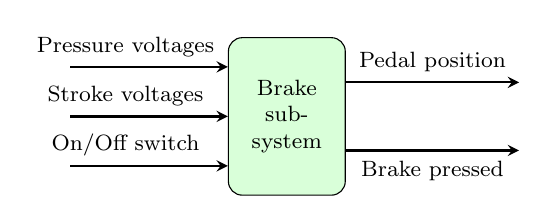
\begin{tikzpicture}
    \tikzstyle{every node} = [font=\footnotesize]
    \tikzstyle{block} = [draw, rectangle, fill=green!15, rounded corners=5pt, minimum width=1 cm, minimum height=2.0 cm]
    % place nodes
    \node[block,text width=1.25cm,text centered](brakeSubsystem){Brake subsystem};

    % Connections
    \draw[stealth-,thick]
    (brakeSubsystem.140)--node[pos=0.65,above]{Pressure voltages}++(-2.0,0);
    \draw[stealth-,thick]
    (brakeSubsystem.180)--node[pos=0.65,above]{Stroke voltages}++(-2.0,0);
    \draw[stealth-,thick]
    (brakeSubsystem.-140)--node[pos=0.65,above]{On/Off switch}++(-2.0,0);
    \draw[-stealth,thick]
    (brakeSubsystem.30)--node[pos=0.5,above]{Pedal position}++(2.2,0);
    \draw[-stealth,thick]
    (brakeSubsystem.-30)--node[pos=0.5,below]{Brake pressed}++(2.2,0);
    
  \end{tikzpicture}
    % \captionsetup{justification=centering, margin=3cm}
    % \includegraphics[width=2.5in]{figs/inkscape/brakeModelArchitecture}
    \caption{Brake subsystem block diagram}
    \label{fig:brakeModelArchitecture}
\end{figure}




%	\centering \includegraphics[width=.45\linewidth]{figs/inkscape/steeringModelArchitecture}\quad%
%	\centering \begin{minipage}[b][0.4\textheight][c]{.45\linewidth} \begin{enumerate} \item Steering System 			\item Brake System \item Acceleration System \end{enumerate} \end{minipage}\\[1em]
%	\centering \includegraphics[width=.45\linewidth]{figs/inkscape/brakeModelArchitecture}\quad%
%	\centering 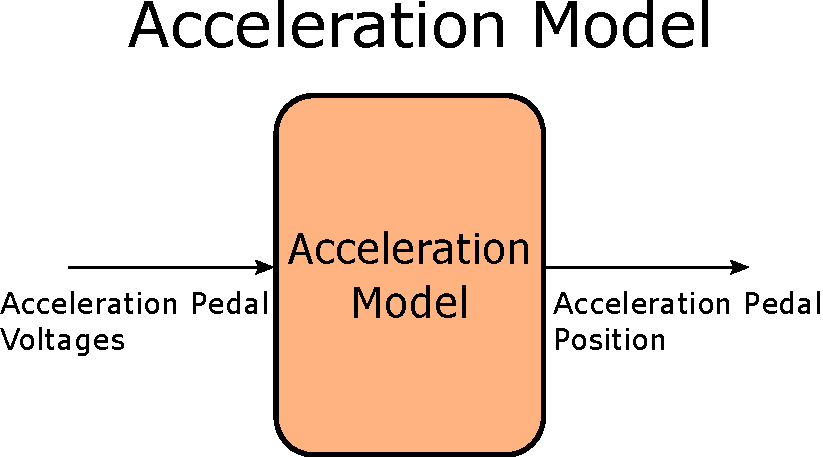
\includegraphics[width=.45\linewidth]{figs/inkscape/accelerationModelArchitecture}
\end{frame}
%
\begin{frame}{System Architecture}{Subsystems}

\begin{figure}[htbp]
    \centering
  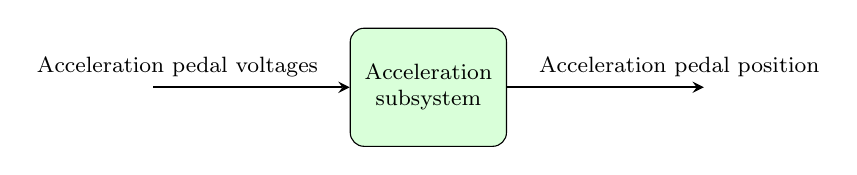
\begin{tikzpicture}
    \tikzstyle{every node} = [font=\footnotesize]
    \tikzstyle{block} = [draw, rectangle, fill=green!15, rounded corners=5pt, minimum width=1.5 cm, minimum height=1.5 cm]
    % place nodes
    \node[block,text width=1.75cm,text centered](accelSubsystem){Acceleration subsystem};
    % Connections
    \draw[stealth-,thick]
    (accelSubsystem.180)--node[very near end,above]{Acceleration pedal voltages}++(-2.5,0);
    \draw[-stealth,thick]
    (accelSubsystem.0)--node[very near end,above]{Acceleration pedal position}++(2.5,0);
  \end{tikzpicture}
    \caption{Acceleration subsystem block diagram}
    \label{fig:accelModelArchitecture}
 \end{figure}
 
 \begin{figure}
    \centering
  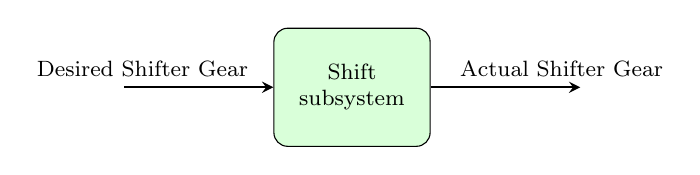
\begin{tikzpicture}
    \tikzstyle{every node} = [font=\footnotesize]
    \tikzstyle{block} = [draw, rectangle, fill=green!15, rounded corners=5pt, minimum width=1.5 cm, minimum height=1.5 cm]
    % place nodes
    \node[block,text width=1.75cm,text centered](shiftSubsystem){Shift subsystem};

    % Connections
    \draw[stealth-,thick]
    (shiftSubsystem.180)--node[very near end,above]{Desired Shifter Gear}++(-1.9,0);
    \draw[-stealth,thick]
    (shiftSubsystem.0)--node[very near end,above]{Actual Shifter Gear}++(1.9,0);
    
  \end{tikzpicture}
    \caption{Shift subsystem block diagram}
    \label{fig:shiftModelArchitecture}
 \end{figure} 

%	\centering 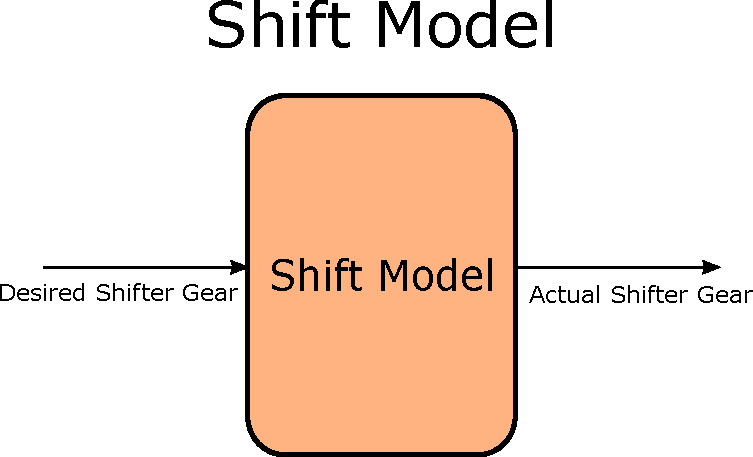
\includegraphics[width=.45\linewidth]{figs/inkscape/shiftModelArchitecture}\quad%
%	\centering \begin{minipage}[b][0.4\textheight][c]{.45\linewidth} \begin{enumerate} \item Shift System \item 		Speed Control System \item Speed System \end{enumerate} \end{minipage}\\[1em]
%	\centering \includegraphics[width=.45\linewidth]{figs/inkscape/speedControlModelArchitecture}\quad%
%	\centering \includegraphics[width=.45\linewidth]{figs/inkscape/speedModelArchitecture}
\end{frame}

\begin{frame}{System Architecture}{Subsystems}
\begin{figure}[htbp]
    \centering
  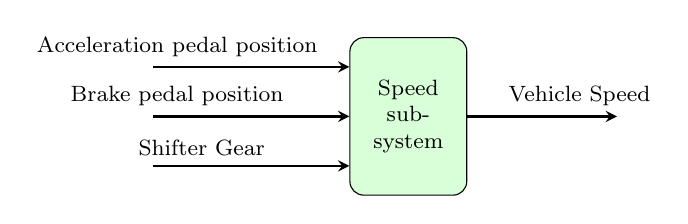
\begin{tikzpicture}
    \tikzstyle{every node} = [font=\footnotesize]
    \tikzstyle{block} = [draw, rectangle, fill=green!15, rounded corners=5pt, minimum width=1 cm, minimum height=2 cm]
    % place nodes
    \node[block,text width=1.25cm,text centered](speedSubsystem){Speed subsystem};

    % Connections
    \draw[stealth-,thick]
    (speedSubsystem.140)--node[very near end,above]{Acceleration pedal position}++(-2.5,0);
    \draw[stealth-,thick]
    (speedSubsystem.180)--node[very near end,above]{Brake pedal position}++(-2.5,0);
    \draw[stealth-,thick]
    (speedSubsystem.-140)--node[near end,above]{Shifter Gear}++(-2.5,0);
    \draw[-stealth,thick]
    (speedSubsystem.0)--node[near end,above]{Vehicle Speed}++(1.9,0);
    
  \end{tikzpicture}
    % \captionsetup{justification=centering, margin=3cm}
    % \includegraphics[width=2.5in]{figs/inkscape/brakeModelArchitecture}
    \caption{Speed subsystem block diagram}
    \label{fig:speedModelArchitecture}
\end{figure}

\begin{figure}[htbp]
    \centering
  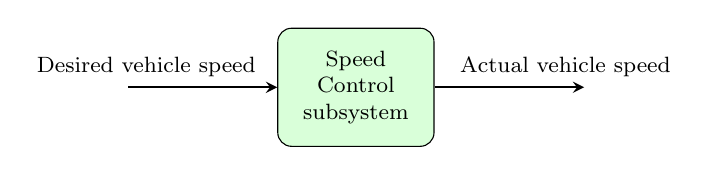
\begin{tikzpicture}
    \tikzstyle{every node} = [font=\footnotesize]
    \tikzstyle{block} = [draw, rectangle, fill=green!15, rounded corners=5pt, minimum width=1.5 cm, minimum height=1.5 cm]
    % place nodes
    \node[block,text width=1.75cm,text centered](speedControlSubsystem){Speed Control subsystem};

    % Connections
    \draw[stealth-,thick]
    (speedControlSubsystem.180)--node[very near end,above]{Desired vehicle speed}++(-1.9,0);
    \draw[-stealth,thick]
    (speedControlSubsystem.0)--node[very near end,above]{Actual vehicle speed}++(1.9,0);
    
  \end{tikzpicture}
    \caption{Speed Control subsystem block diagram}
    \label{fig:speedControlModelArchitecture}
 \end{figure}

\end{frame}

%---------------------------
\section{System Modeling using Neural Networks}

\begin{frame}{Modeling using Neural Networks}{}
  \begin{figure}
    \centering
    \tikzset{%
      input neuron/.style={
        circle,
        fill=green!50,
        minimum size=0.7cm
      },
      neuron missing/.style={
        draw=none, 
        scale=1,
        fill=white,
        text height=0.01cm,
        execute at begin node=\color{black}$\vdots$
      },
    }

    \tikzset{%
      hidden neuron/.style={
        circle,
        fill=blue!50,
        minimum size=0.7cm
      },
      neuron missing/.style={
        draw=none, 
        scale=1,
        fill=white,
        text height=0.01cm,
        execute at begin node=\color{black}$\vdots$
      },
    }

    \tikzset{%
      output neuron/.style={
        circle,
        fill=red!50,
        minimum size=0.7cm
      },
      neuron missing/.style={
        draw=none, 
        scale=1,
        fill=white,
        text height=0.01cm,
        execute at begin node=\color{black}$\vdots$
      },
    }      

    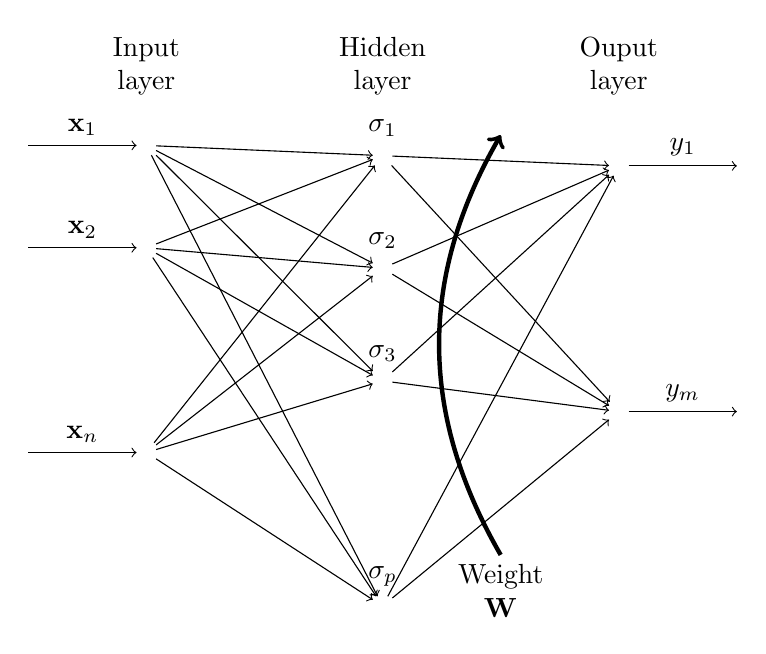
\begin{tikzpicture}[x=1.5cm, y=1.3cm,transform shape]

      \foreach \m/\l [count=\y] in {1,2,missing,3}
      \node [input neuron/.try, neuron \m/.try] (input-\m) at (0,2.5-\y) {};

      \foreach \m [count=\y] in {1,2,3,missing,4}
      \node [hidden neuron/.try, neuron \m/.try ] (hidden-\m) at (2,2.5-\y*1.1) {};

      \foreach \m [count=\y] in {1,missing,2}
      \node [output neuron/.try, neuron \m/.try] (output-\m) at (4,2.5-\y*1.2) {};

      \foreach \l [count=\i] in {1,2,n}
      \draw [<-] (input-\i) -- ++(-1,0)
      node [above, midway] {$\mathbf{x}_{\l}$};

      \foreach \l [count=\i] in {1,2,3,p}
      \node [above] at (hidden-\i.north) {$\sigma_{\l}$};

      \foreach \l [count=\i] in {1,m}
      \draw [->] (output-\i) -- ++(1,0)
      node [above, midway] {${y}_{\l}$};

      \foreach \i in {1,...,3}
      \foreach \j in {1,...,4}
      \draw [->] (input-\i) -- (hidden-\j);

      \foreach \i in {1,...,4}
      \foreach \j in {1,2}
      \draw [->] (hidden-\i) -- (output-\j);



      \foreach \l [count=\x from 0] in {Input, Hidden, Ouput}
      \node [align=center, above] at (\x*2,1.9) {\l \\ layer};

      \node [align=center, below] at (3,-2.5) {Weight \\ $\mathbf{W}$};
      \draw[->,ultra thick](3,-2.5) to[bend left] (3,1.6);

    \end{tikzpicture}
    \caption{Neural network structure for approximating system behavior}
    \label{fig:nnActor}
		\end{figure}
\end{frame}

%\begin{frame}
%
%  Therefore, approximated output signal can be written as:
%\begin{align}
%  \label{eq:approximatePolicyActorWeights}
%    \mathbf{y} = \mathbf{W}^T\bm{\sigma}(\mathbf{x}),
%  \end{align}
%%
%where $\bm{\sigma}:\mathbb{R}^n\to\mathbb{R}^{p}$ with components of weight matrix ${\bf W}$ shown in Fig.~\ref{fig:nnActor} are given by %
%%
%\begin{align*}
%  {\bf W} = 
%  \begin{bmatrix}
%    w^{1,1} &  w^{1,2} & \ldots &w^{1,m}\\
%    w^{2,1} & w^{2,2}& \ldots &w^{1,m}\\
%    \vdots & \ddots & \ldots &\vdots\\
%    w^{p,1} & w^{p,2}& \ldots &w^{p,m}
%  \end{bmatrix}.
%\end{align*}
%%
%
%Now take $\eta$ data points and form the set of linear equations as: %
%%
%\begin{align*}
%&  \bm{\sigma}^T(\mathbf{x}_k) \mathbf{W}  \approx     \left(\mathbf{y}_{k}^{[d]}\right)^T\\
% & \bm{\sigma}^T(\mathbf{x}_{k+1}) \mathbf{W}  \approx     \left(\mathbf{y}_{k+1}^{[d]}\right)^T\\
%                                            &\vdots \\
% & \bm{\sigma}^T(\mathbf{x}_{k+\eta-1}) \mathbf{W}  \approx     \left(\mathbf{y}_{k+\eta-1}^{[d]}\right)^T  
%\end{align*}
%%
%\end{frame}


%\begin{frame}
%  In compact form:
%  \begin{align*}
%    \bm{\Sigma}\mathbf{W} \approx  \mathbf{U}^{[d]},\qquad\text{with}
%    % \hat{\mathbf{U}} \approx \mathbf{U}^{[d]}, 
%  \end{align*}
%  %
%  $\mathbb{R}^{\eta\times p}\ni \bm{\Sigma} = [\bm{\Sigma}_0,\bm{\Sigma}_1,\ldots,\bm{\Sigma}_{\eta -1}]^T$ with $\bm{\Sigma}_\kappa = \bm{\sigma}^T({\bf x}_{k+\kappa})$ and $\mathbb{R}^{\eta\times m}\ni {\bf U}^{[d]} = [{\bf U}_0,{\bf U}_1,\ldots, {\bf U}_{\eta-1}]^T$ with ${\bf U}_\kappa = \left({\bf y}_{\kappa}\right)^T$ for $\kappa = 0,1,\ldots,\eta-1.$
%
%  Let $\bm{\Sigma}\mathbf{W}\equiv \hat{\mathbf{U}},$ sum-of-squared error, $\delta$ can be written as:
%  \begin{align*}
%    \delta = \frac{1}{2}\|\mathbf{U}^{[d]} - \hat{\mathbf{U}}\|^2
%  \end{align*}
%
%Weight matrix ${\bf W}$ can then be found minimizing the sum--of--square error $\delta$ defined by %
%%
%\begin{align*}
%  \delta = \frac{1}{2}\|{\bf U}^{[d]} - \bm{\Sigma} {\bf W}\|^2  = \frac{1}{2}\mathrm{Tr}\left[({\bf U}^{[d]} - \bm{\Sigma} {\bf W})^T({\bf U}^{[d]} - \bm{\Sigma} {\bf W})\right].
%\end{align*}
%%
%Taking the derivative of $\delta$ with respect to ${\bf W}$ yields 
%%
%\begin{align}
%  \frac{\partial\delta}{\partial\mathbf{W}} = - \bm{\Sigma}^T\mathbf{U}^{[d]} + \bm{\Sigma}^T \bm{\Sigma}\mathbf{W}
%  \label{eq:actorWeightsGradient}
%\end{align}
%%
%
%\end{frame}

%\begin{frame}
%
%
%  Setting $\frac{\partial\delta}{\partial\mathbf{W}}$ to zero yields
%  \begin{align*}
%    {\bf W} = \left(\bm{\Sigma}^T\bm{\Sigma}\right)^T\bm{\Sigma}^T{\bf U}^{[d]}.
%  \end{align*}
%  
%$\bullet$ Hidden layer to output layer weight is updated at each policy iteration $r=0,1,\ldots$ using gradient descent approach as:
%
%\begin{multline}
%  \mathbf{W}^{(r+1)} = \mathbf{w}^{(r)} - \ell\frac{\partial\delta}{\partial\mathbf{W}}= \mathbf{W}^{(r)} - \ell\left(-\bm{\Sigma}^T\mathbf{U}^{[d]} + \bm{\Sigma}^T \bm{\Sigma}\mathbf{W}^{(r)}\right)\\
%  = \mathbf{w}^{(r)}-\ell \bm{\Sigma}^T\left(\bm{\Sigma}\mathbf{W}^{(r)} - \mathbf{U}^{[d]}\right)
%  \label{eq:actorWeightUpdate}
%\end{multline}
%
%\end{frame}

\begin{frame}{Modeling using Neural Networks}{}
	\begin{block}{}
 \begin{itemize}
        \item Used MATLAB's Neural Network Time Series App 
        \item All models generated using the Bayesian Regularization Algorithm 
        \item Models trained using collected log data 
\end{itemize}
  \end{block}
\end{frame}

%-------------------------
\section{Modeling Vehicle Subsystems}

\begin{frame}{Modeling Vehicle Subsystems}{System Requirements}
	\begin{block}{Specifications}
	\begin{minipage}[t]{0.62\linewidth}    
    Proposed vehicle subsystem models are expected to fulfill requirements listed below:
	\begin{itemize}
    		\item Resulting plant model will consist of reasonably accurate subsystem models
    		\item Subsystems can be used to create a HIL testbench
    		\item Steering model can handle very small changes in steering angles
    \begin{itemize}
		\item smooth out any non-linear discontinuities that would normally be measured by the steering motor, especially for small changes in the steering angle, depicted in \autoref{fig:nonlinGraph}.
    \end{itemize}
	\end{itemize}
	\end{minipage}
	\begin{minipage}[t]{0.34\linewidth}
	\begin{figure}[h]
		\centering
    		\captionsetup{justification=centering, margin=0.5cm}
    		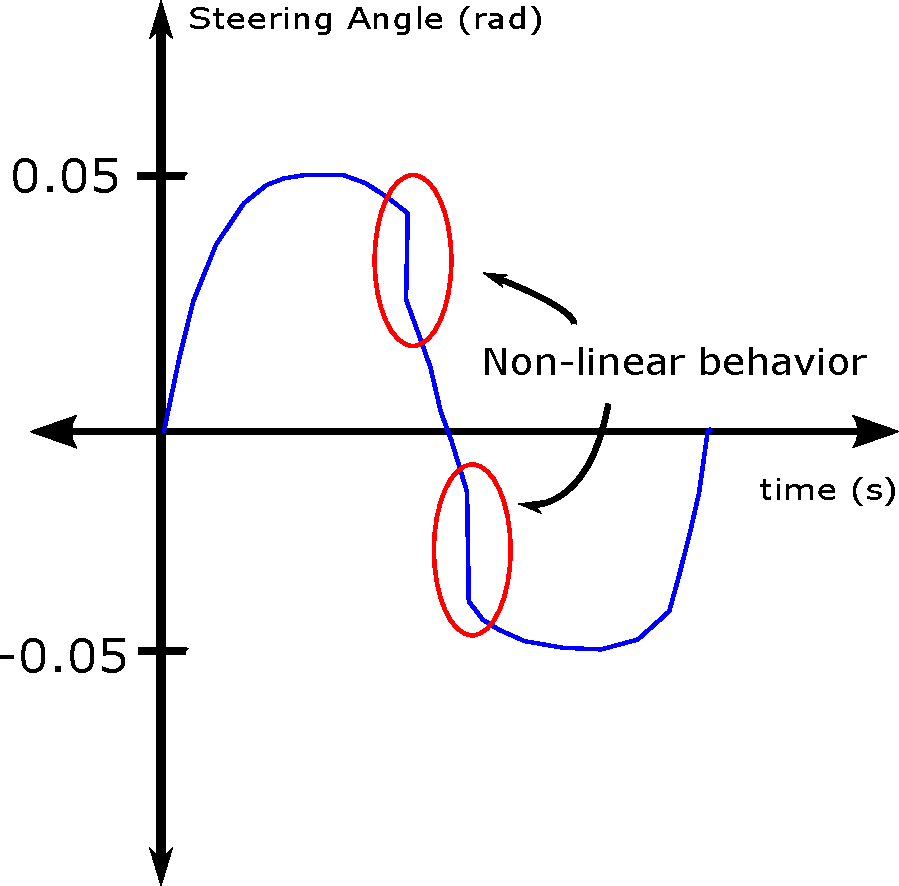
\includegraphics[width=1.5in]{figs/inkscape/nonlinearBehavior}
    		\caption{Steering Non-linear Behavior}
    		\label{fig:nonlinGraph}
	\end{figure}
	\end{minipage}
\end{block}
\end{frame}
%-------------------------

\section{Simulation Results}

\begin{frame}{Transfer Function Modeling}{Steering System Simulation}
	\begin{block}{Manual Mode}
 		\begin{figure}
		    \centering
		    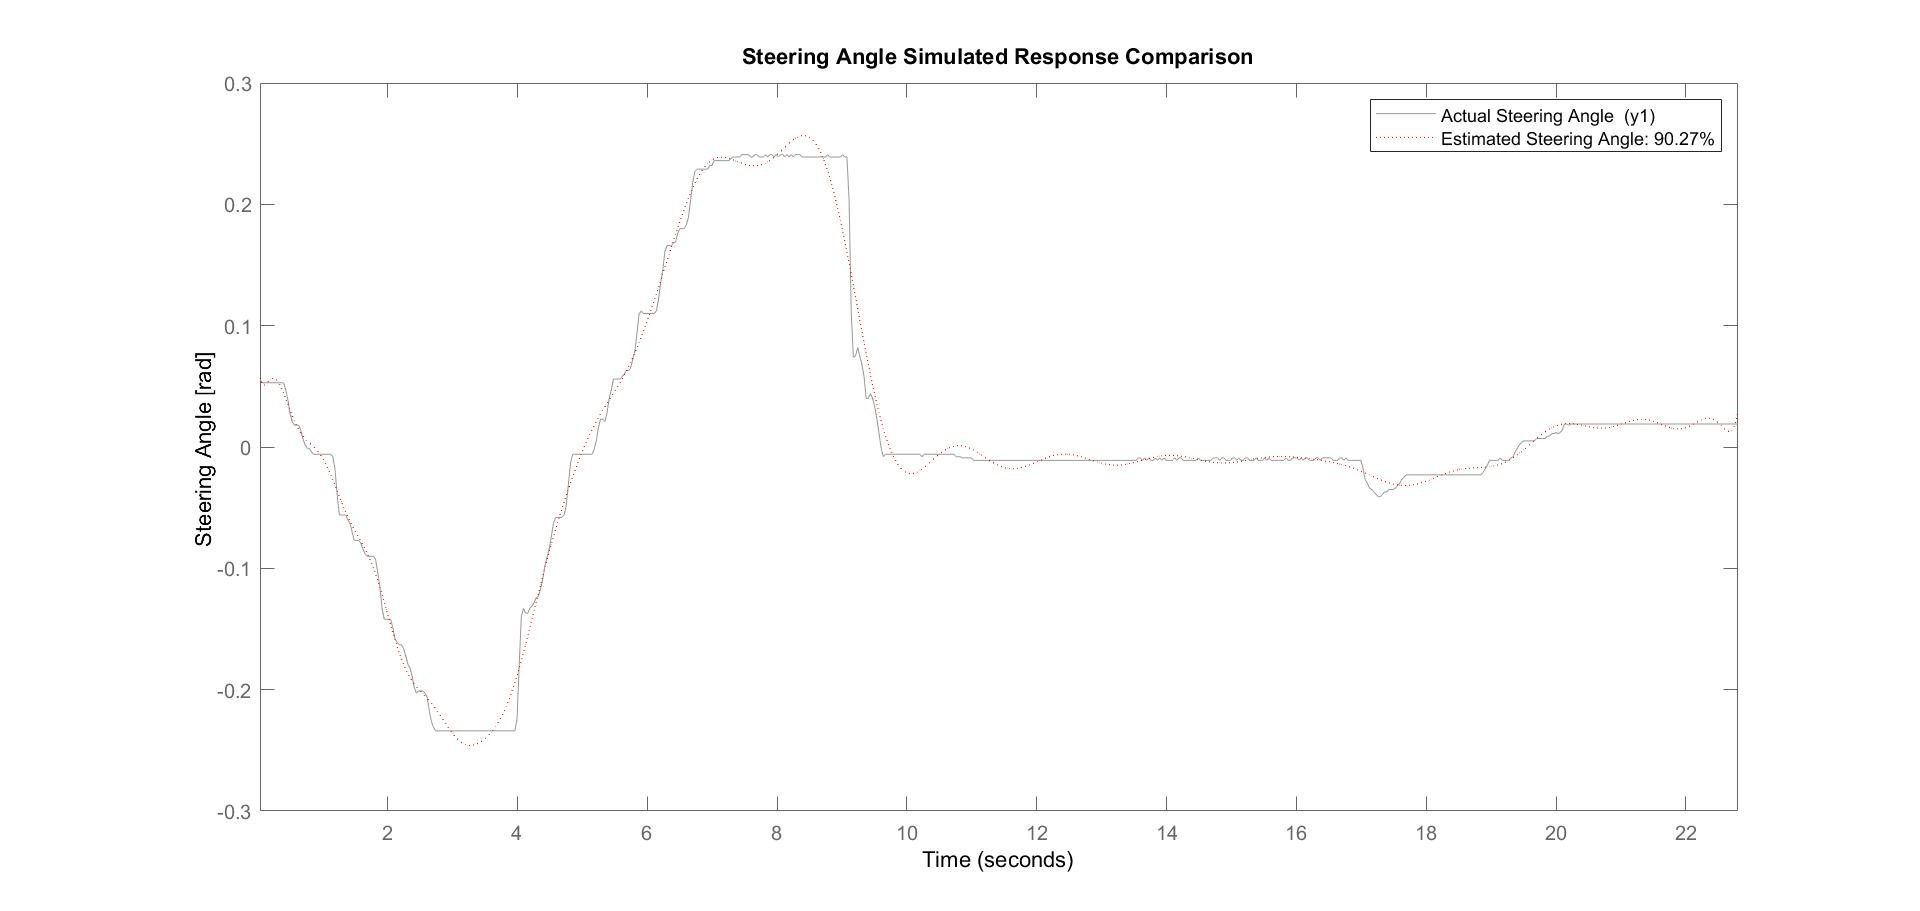
\includegraphics[width=0.4\textwidth]{figs/img/byWireSteeringTransferFunctionModel}
		    \caption{Output of Estimated Manual System Model}
		        \label{fig:manualSteerModel}
 		\end{figure}
  	\end{block}
\end{frame}

\begin{frame}{Transfer Function Modeling}{Steering System Simulation (Cont.)}
	\begin{block}{By-Wire Mode}
		\begin{figure}
    			\centering
    			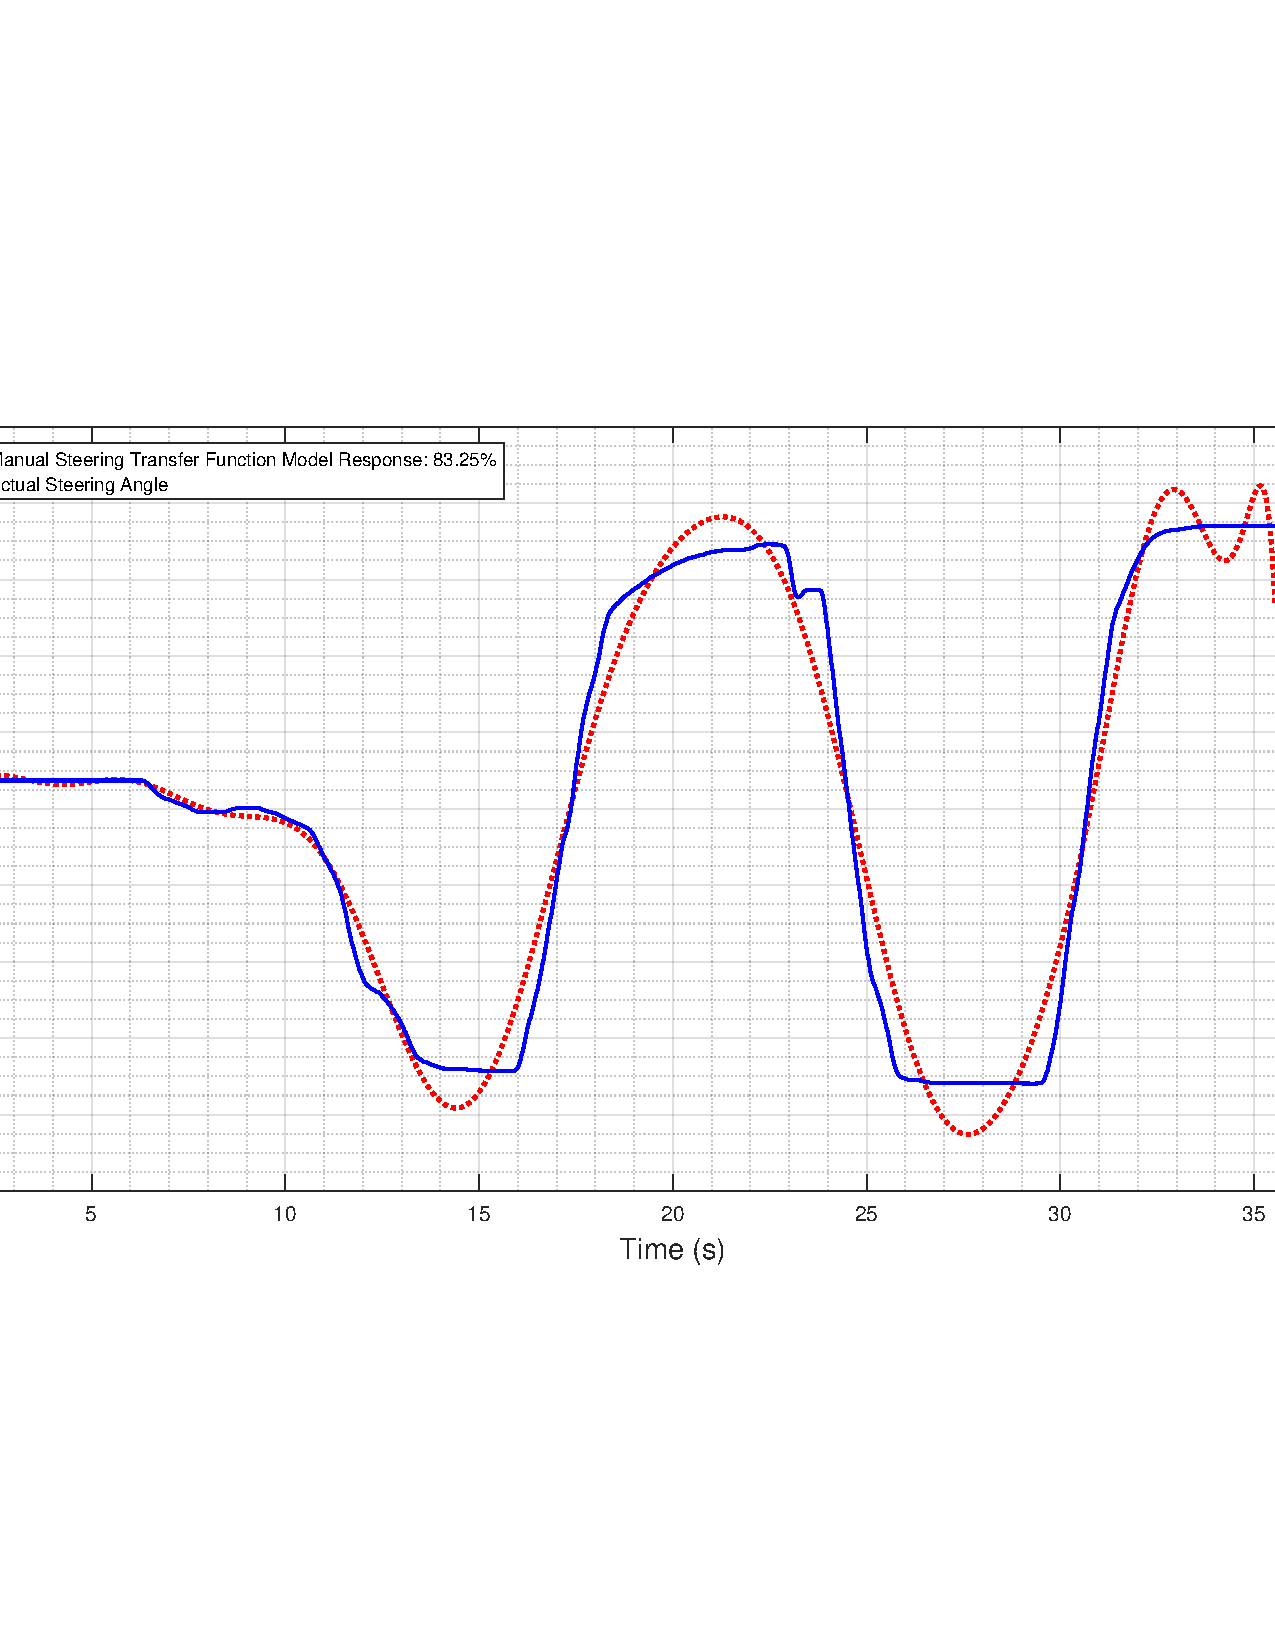
\includegraphics[width=0.4\textwidth]{figs/img/manualSteeringTransferFunctionModel}
    			\caption{Output of Estimated By-Wire System Model}
        		\label{fig:byWireSteerModel}
 		\end{figure}
	\end{block}
\end{frame}

%-------------------------
\begin{frame}{Transfer Function Modeling}{Acceleration System Simulation}
	\begin{block}{Manual Mode}
 		\begin{figure}
	    		\centering
	    		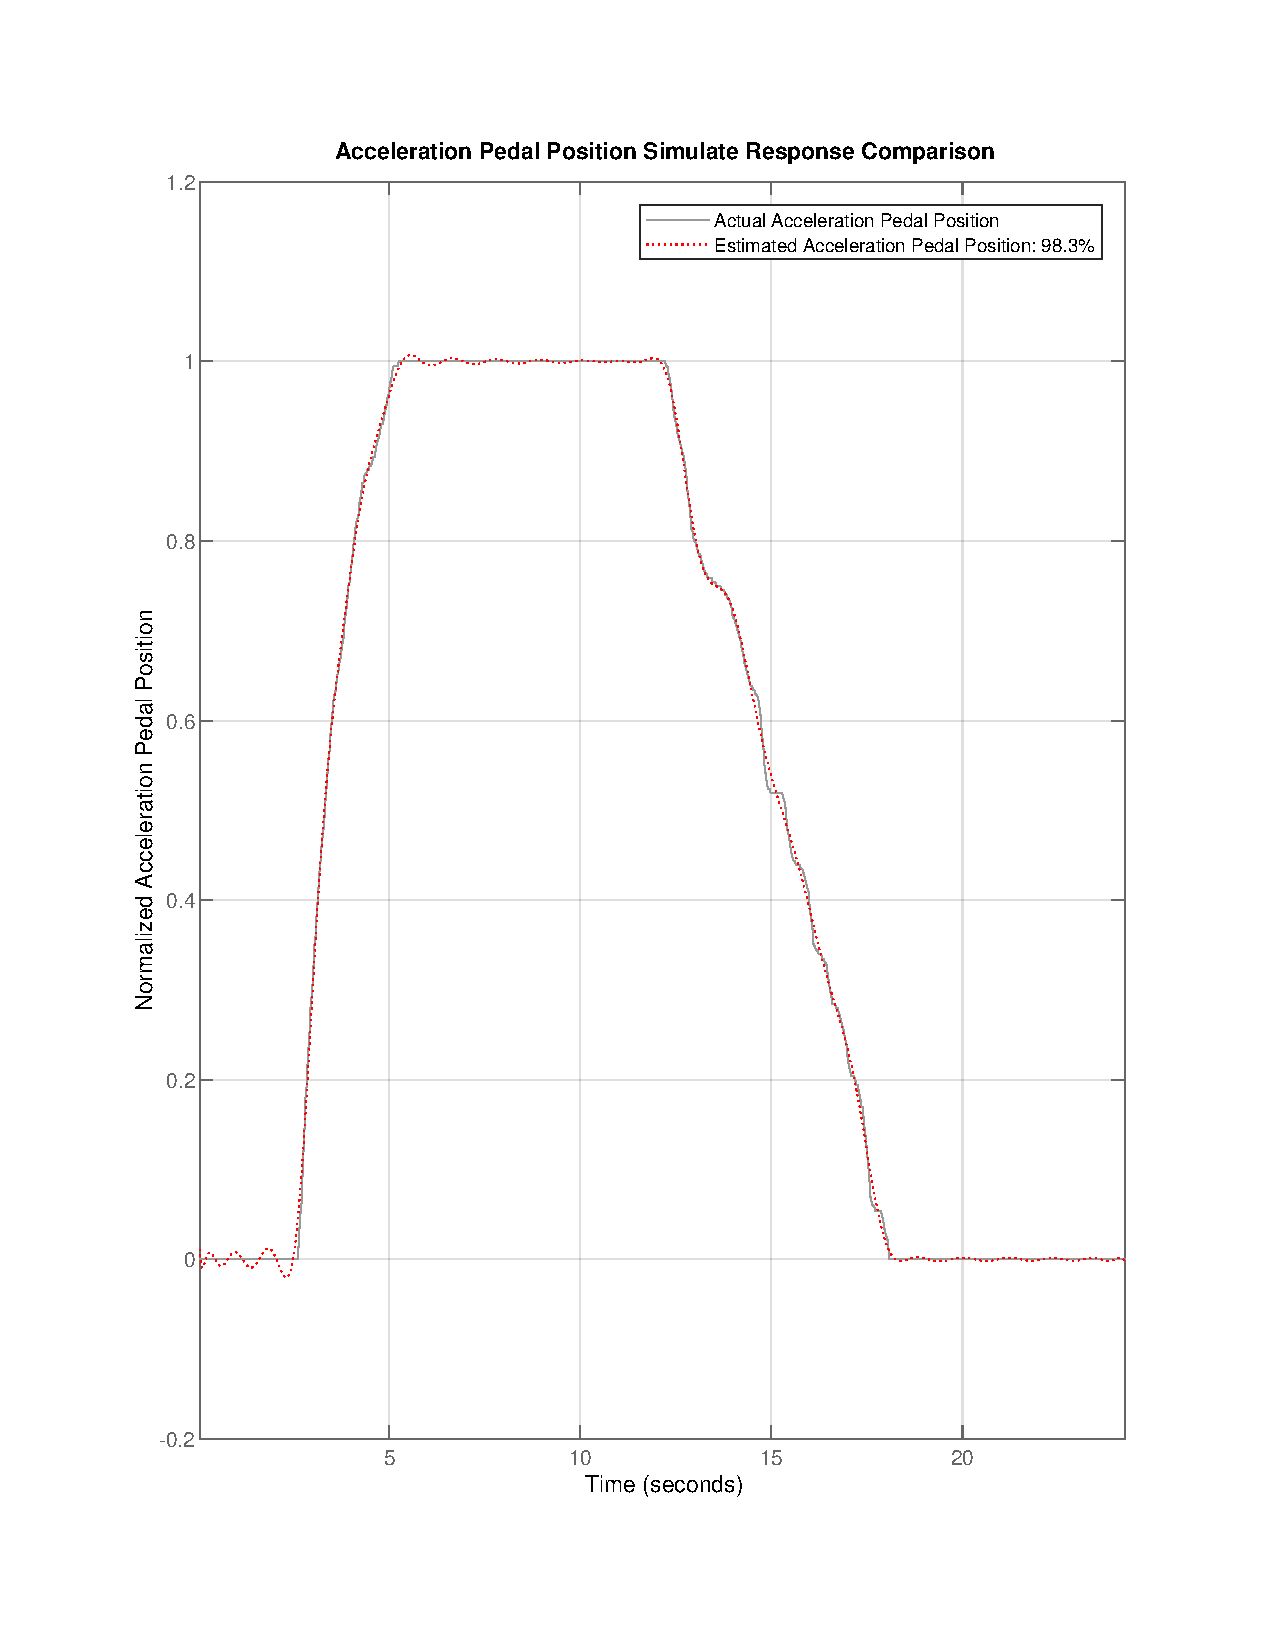
\includegraphics[width=0.4\textwidth]{figs/img/manualAccelTransferFunctionModel}
	        \caption{Output of Estimated Manual System Model}
	        \label{fig:manualAccelModel}
		\end{figure}
  	\end{block}
\end{frame}

\begin{frame}{Transfer Function Modeling}{Acceleration System Simulation (Cont.)}
	\begin{block}{By-Wire Mode}
		\begin{figure}
    			\centering
    			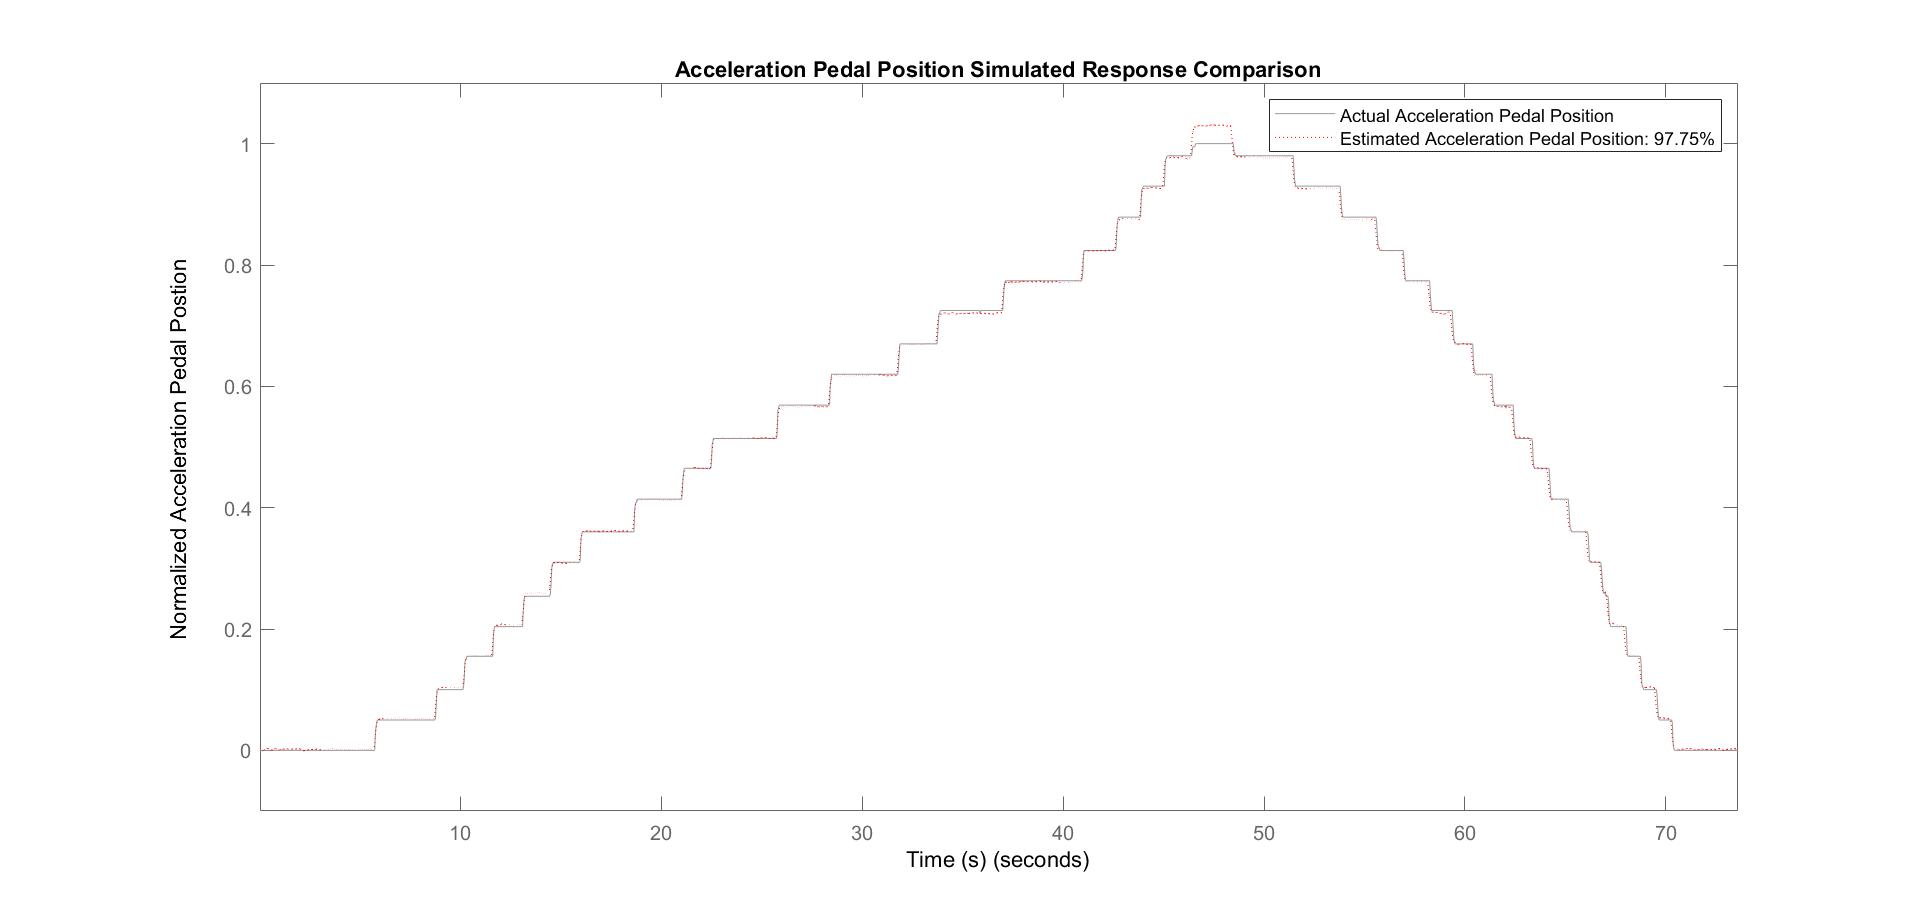
\includegraphics[width=0.4\textwidth]{figs/img/byWireAccelArxModel}
    			\caption{Output of Estimated By-Wire System Model}
        		\label{fig:byWireSteerModel}
 		\end{figure}
	\end{block}
\end{frame}

%-------------------------
\begin{frame}{Transfer Function Modeling}{Brake System Simulation}
	\begin{block}{}
 		\begin{itemize}
			\item Only manual models were considered 
			\item There were no transfer function models that could satisfy both the best fit and error requirements 
 		\end{itemize}
  	\end{block}
\end{frame}

%-------------------------
\begin{frame}{Neural Network Modeling}{Steering System Simulation}
	\begin{block}{}  		
  		\begin{figure}[H]
  			\centering 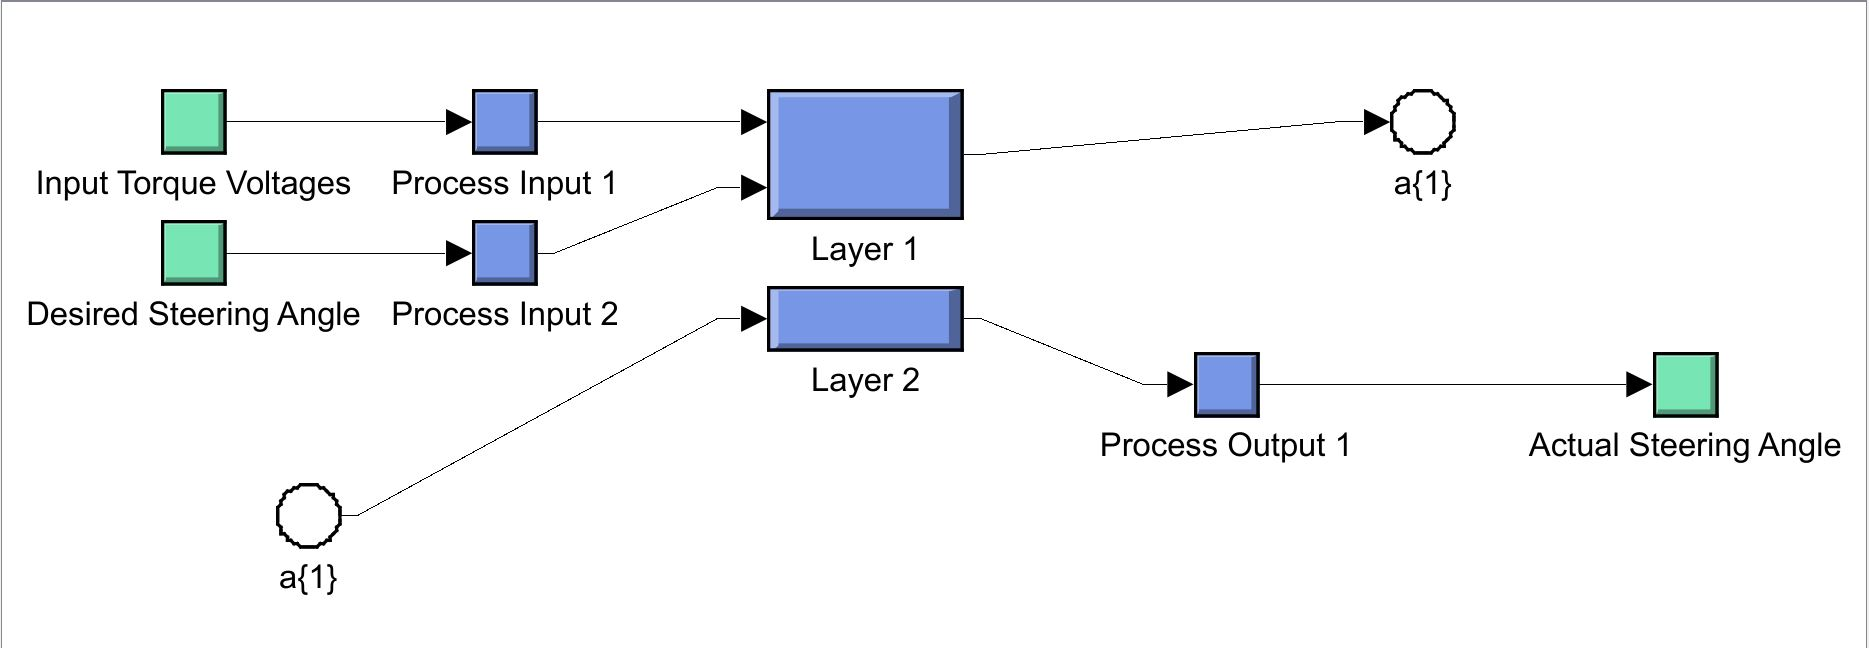
\includegraphics[width=.45\linewidth , height=.37\textheight]{figs/img/steeringSimulinkBlock.jpg}\quad%
			\centering \begin{minipage}[b][0.4\textheight][c]{.45\linewidth}  \begin{itemize}
			\item Only a few samples are just outside of the accuracy requirements
			\item Transfer function model did not meet the accuracy requirements
			\end{itemize} \end{minipage}\\[1em]
			\centering 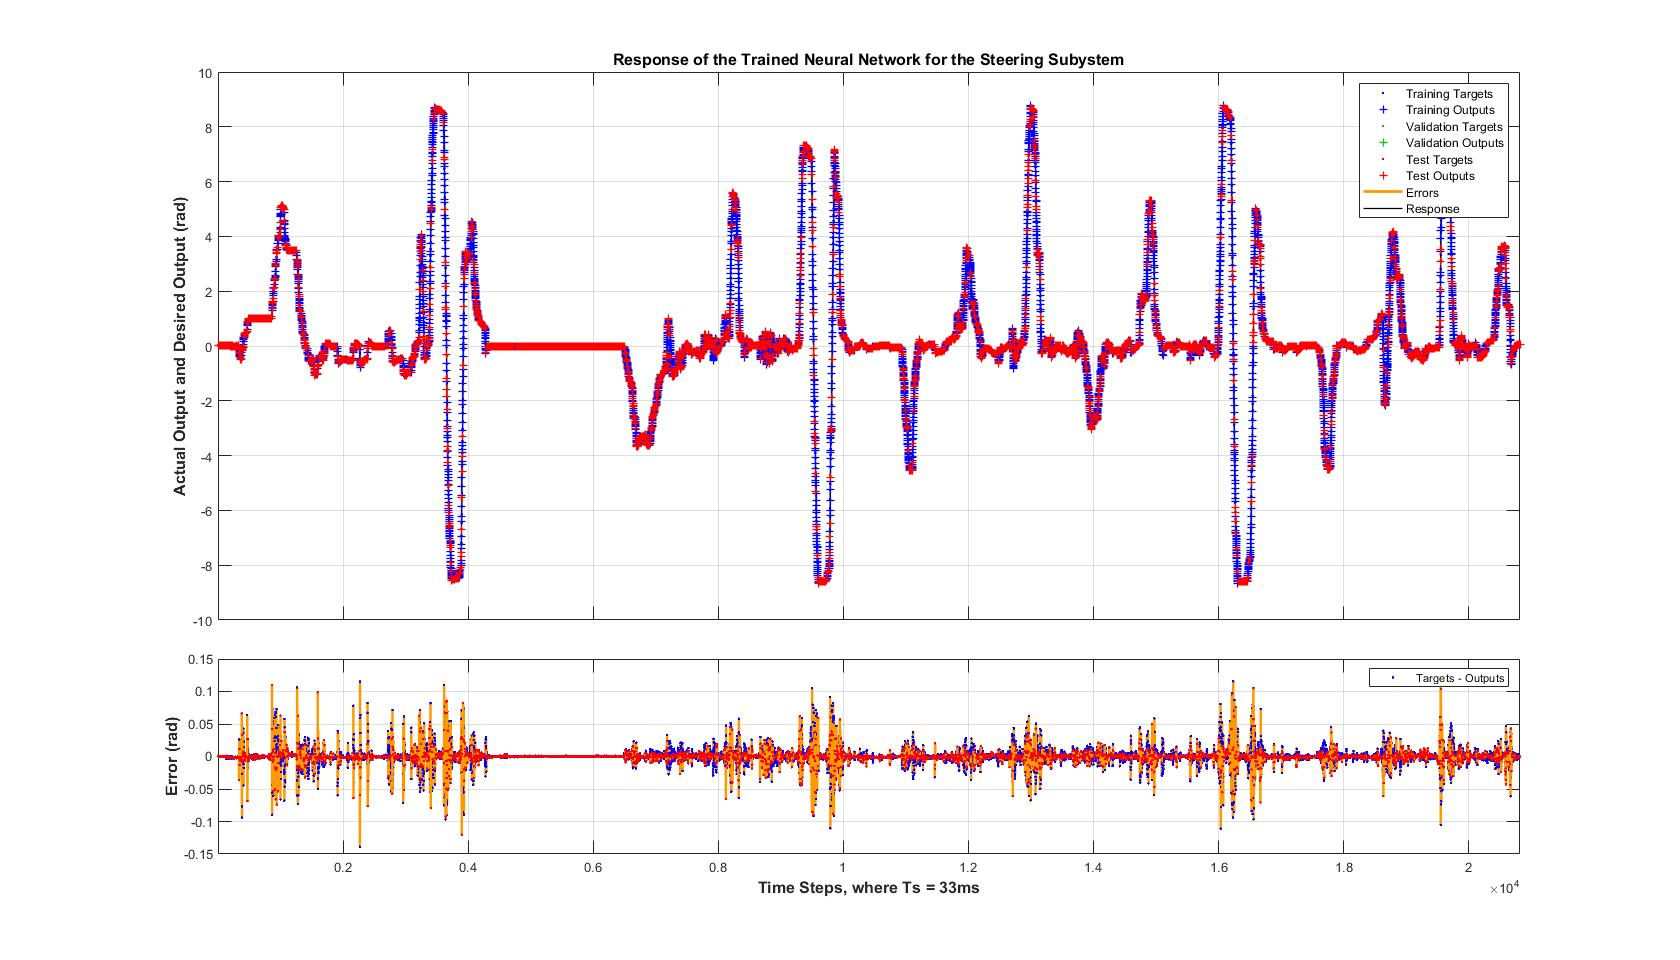
\includegraphics[width=.45\linewidth , height=.37\textheight]{figs/img/steeringNeuralNetworkTrainedOutput.jpg}\quad%
			\centering 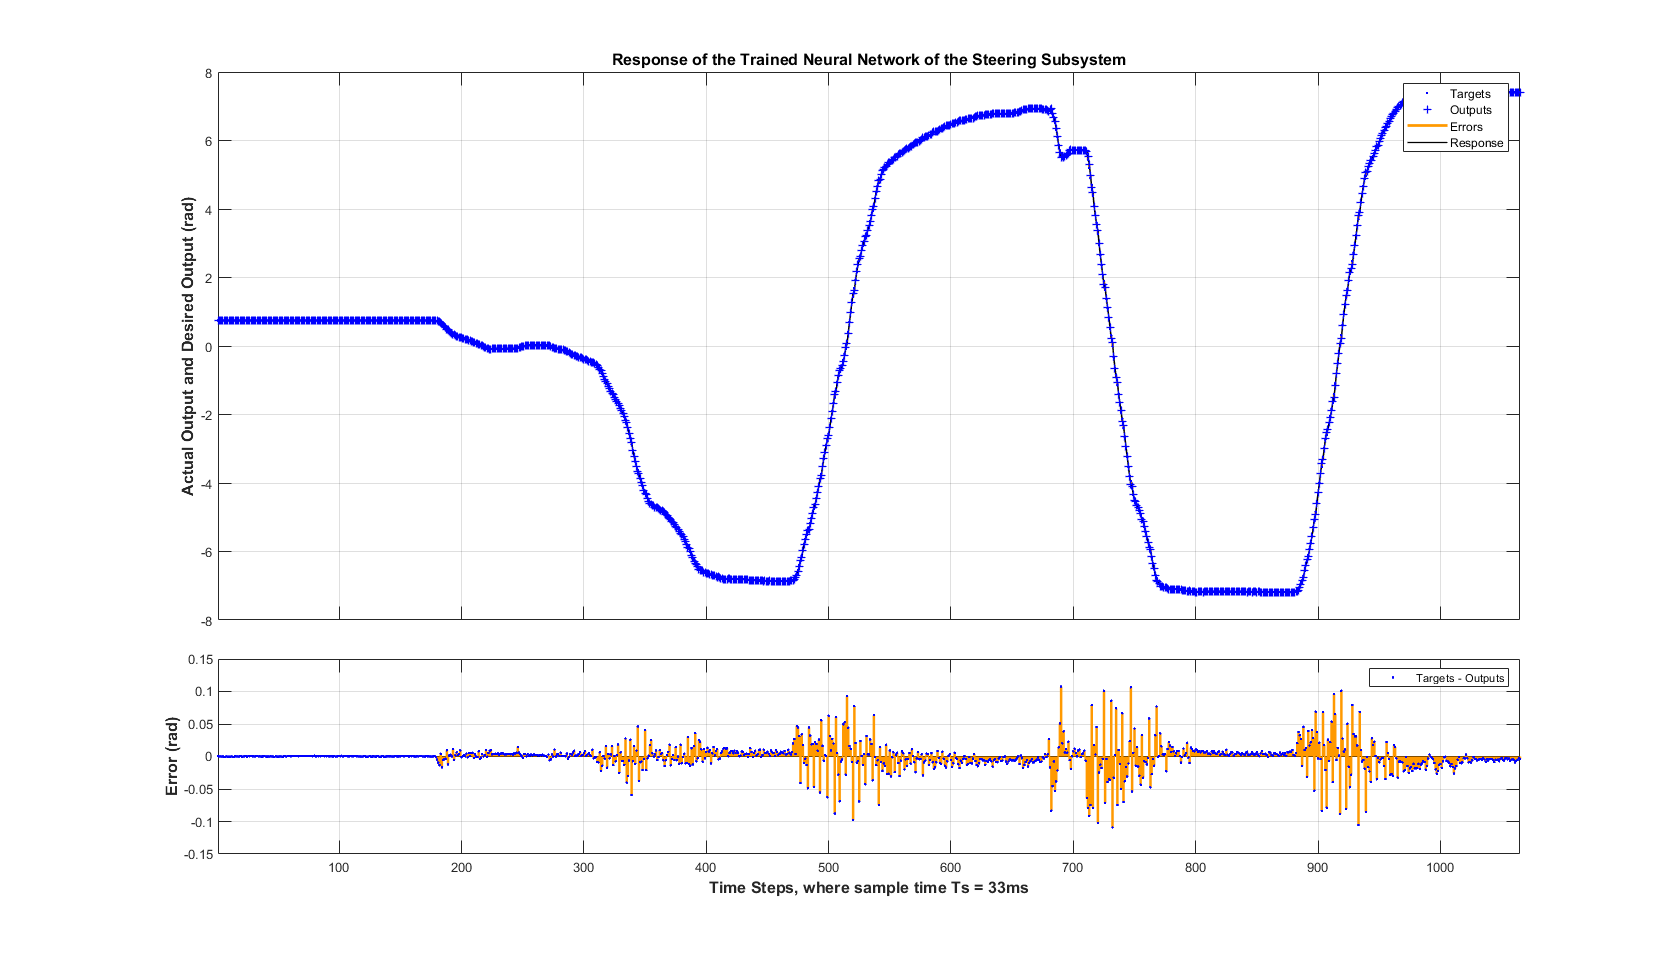
\includegraphics[width=.45\linewidth , height=.37\textheight]{figs/img/steeringNeuralNetworkTrainedOutput2.jpg}
  		\end{figure}
	\end{block}
\end{frame}
%-------------------------
\begin{frame}{Neural Network Modeling}{Acceleration System Simulation}
	\begin{block}{}
  		\begin{figure}[H]
  			\centering 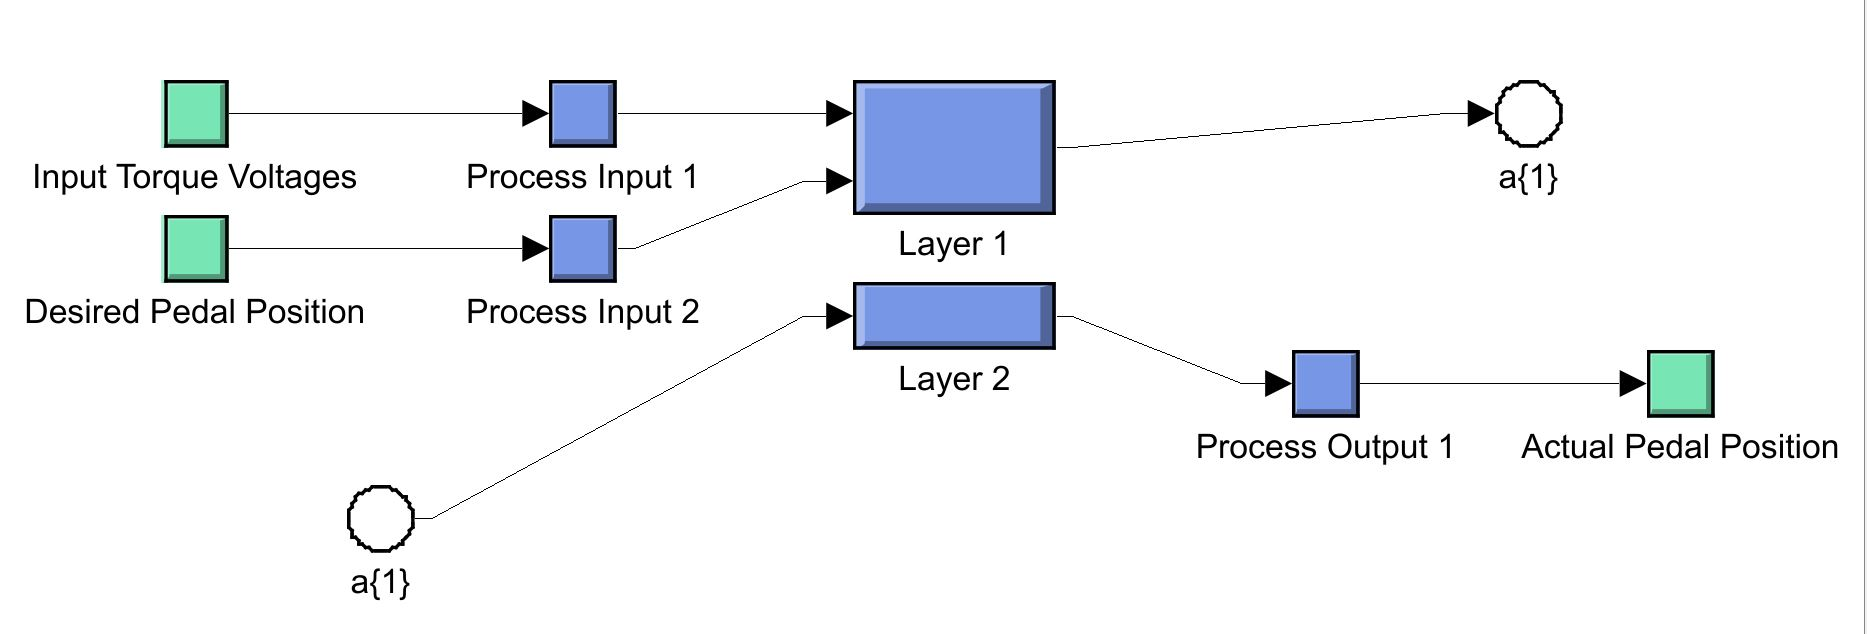
\includegraphics[width=.45\linewidth , height=.37\textheight]{figs/img/accelerationSimulinkBlock.jpg}\quad%
			\centering \begin{minipage}[b][0.4\textheight][c]{.45\linewidth}  \begin{itemize}
			\item All samples within 2\% of the actual output
			\item Transfer function model did not have the same accuracy bounds
			\item Fewer concerns about connections in Simulink
			\end{itemize} \end{minipage}\\[1em]
			\centering 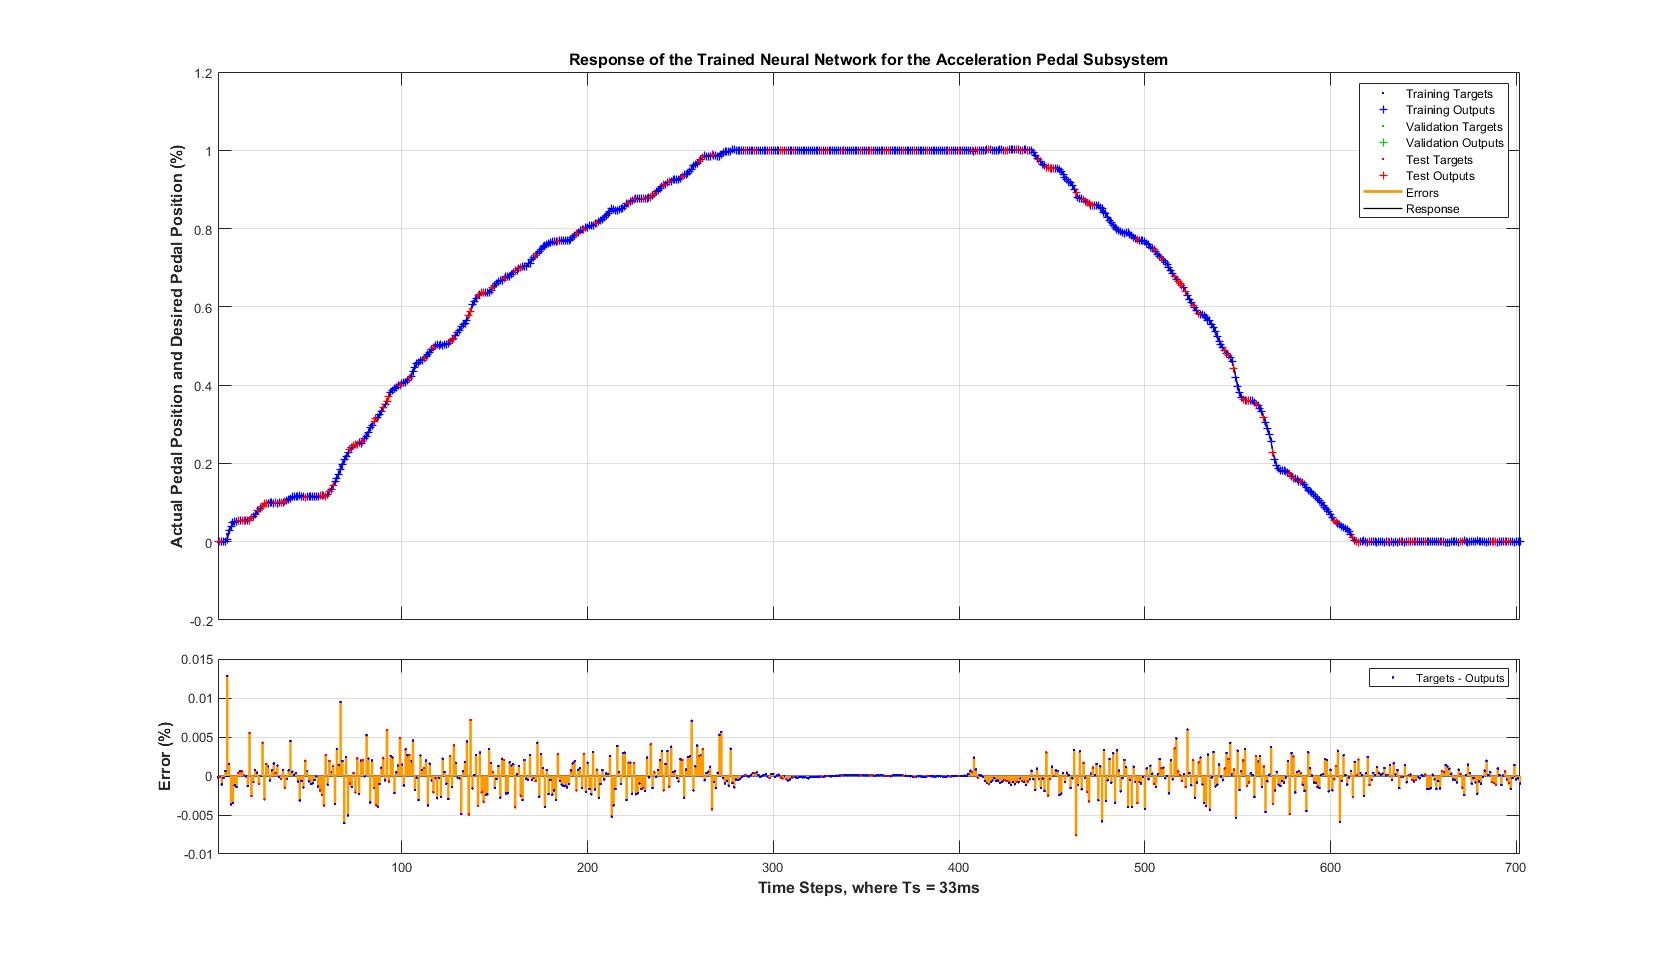
\includegraphics[width=.45\linewidth , height=.37\textheight]{figs/img/accelNeuralNetworkTrainedOutput.jpg}\quad%
			\centering 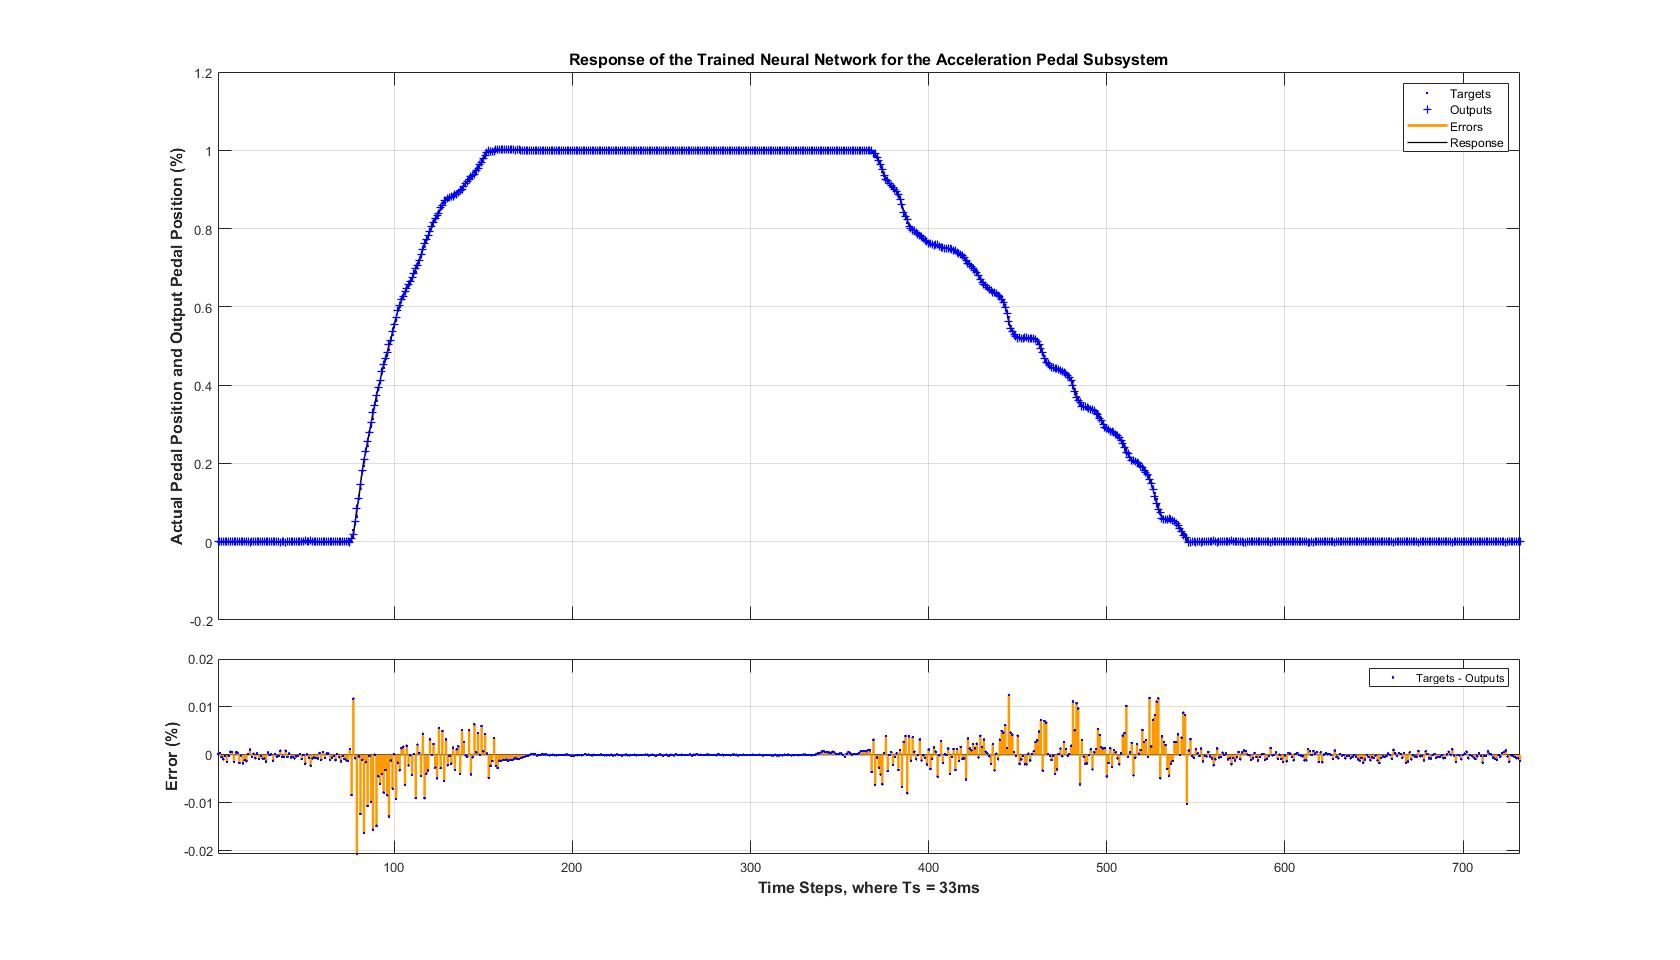
\includegraphics[width=.45\linewidth , height=.37\textheight]{figs/img/accelNeuralNetworkTrainedOutput2.jpg}
  		\end{figure}
	\end{block}
\end{frame}
%-------------------------
\begin{frame}{Neural Network Modeling}{Brake System Simulation}
	\begin{block}{}
\begin{figure}[H]
  			\centering 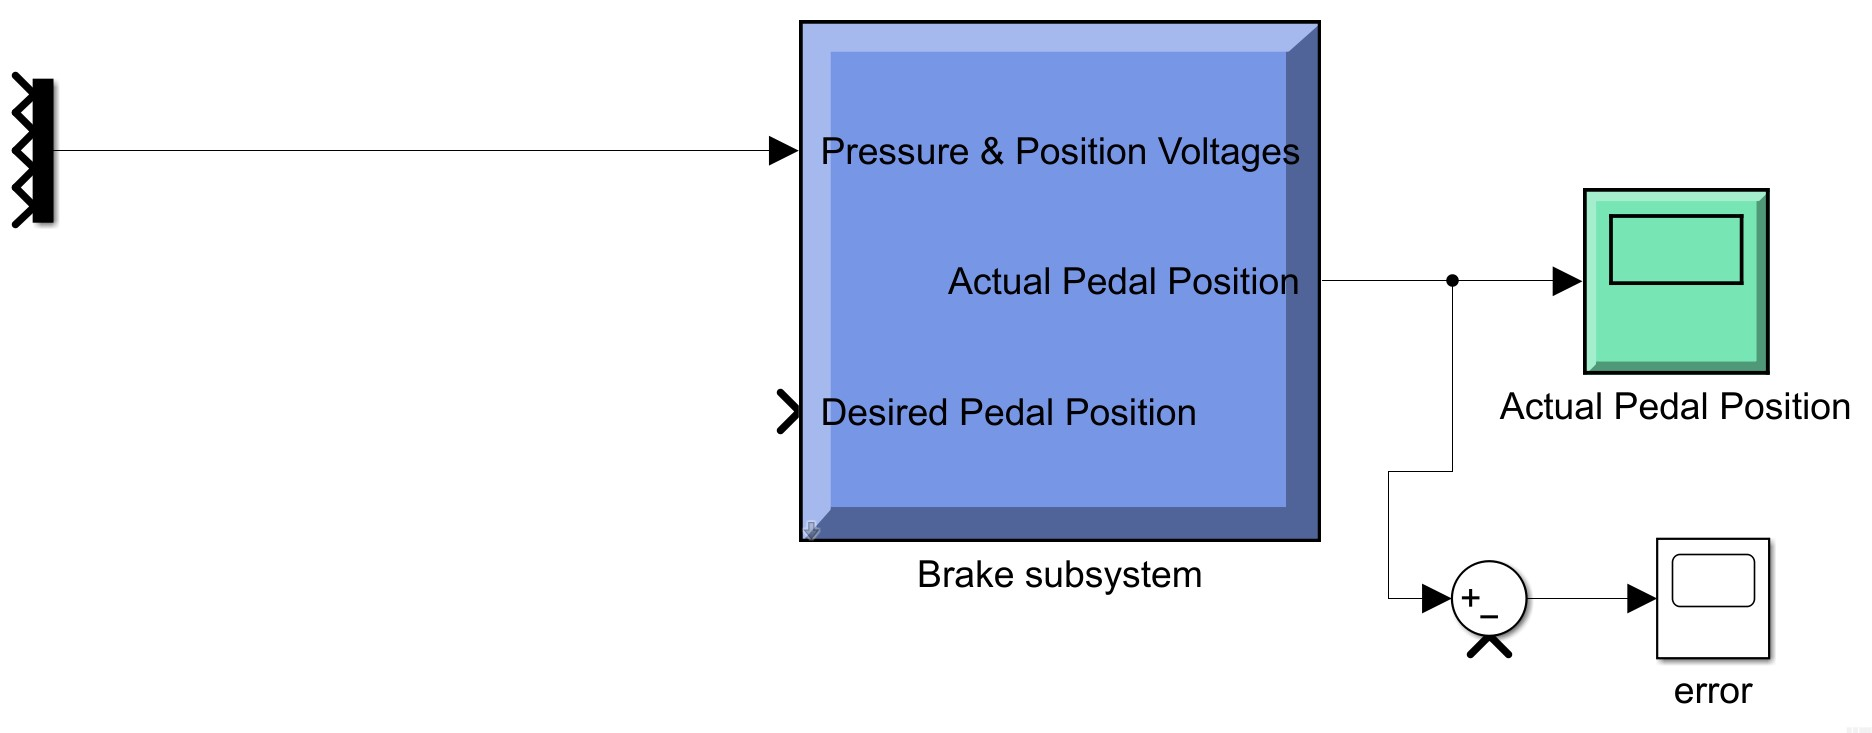
\includegraphics[width=.48\linewidth , height=.37\textheight]{figs/img/brakeSimulinkBlock}\quad%
			\centering \begin{minipage}[b][0.4\textheight][c]{.45\linewidth}  \begin{itemize}
			\item With this model, the error is kept below 5\%
			\item Able to easily track model performance
			\item Provides better results than the transfer function model
			\end{itemize} \end{minipage}\\[1em]
			\centering 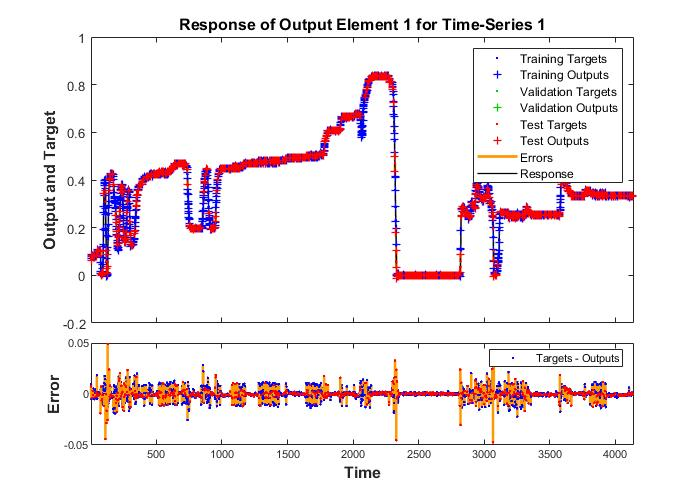
\includegraphics[width=.45\linewidth , height=.37\textheight]{figs/img/brake_new_neuralNetworkFig.jpg}\quad%
			\centering 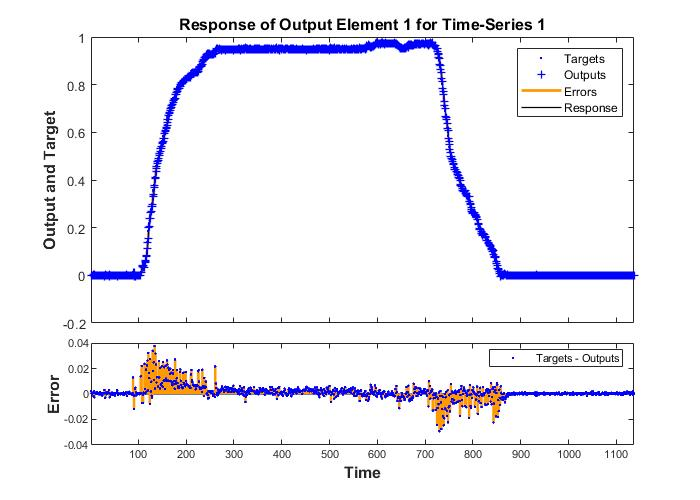
\includegraphics[width=.45\linewidth , height=.37\textheight]{figs/img/brake_new_neuralNetworkFigLog2Test.jpg}
  		\end{figure}
	
  \end{block}
\end{frame}
%-------------------------
\section{Validation and Testing}

\begin{frame}{Validation and Testing}{Experimental Setup}
  \begin{block}{Software and Hardware}
 \begin{itemize}
        \item Software
        \begin{itemize}
	        \small
	        \item MATLAB's System Identification Toolbox
	        \item MATLAB's Neural Network Time Series Toolbox
	        \item DSpace/Control Desk
	        \item Vector CANAlyzer
        \end{itemize}
	\item Hardware
	\begin{itemize}
		\small
		\item Laptop
		\item PACMod ECU
		\item CANCase 
		\item CAN bus
	\end{itemize}
\end{itemize}
  \end{block}
\end{frame}

\begin{frame}{Validation and Testing}{Experimental Setup}
	\begin{block}{Control Method}
		\begin{itemize}
			\item Manual Mode
			\begin{itemize}
				\item Vehicle is not autonomous
				\item Torque voltages are sent by the vehicle ECU
			\end{itemize}
			\item By-Wire Mode
			\begin{itemize}
				\item Vehicle is autonomous
				\item Torque voltages are sent by the PACMod ECU
				\item Torque voltages sent from the vehicle ECU are discarded by open-circuiting the motors
			\end{itemize}
		\end{itemize}
		\begin{figure}
			\centering
    			\captionsetup{justification=centering, margin=3cm}
    			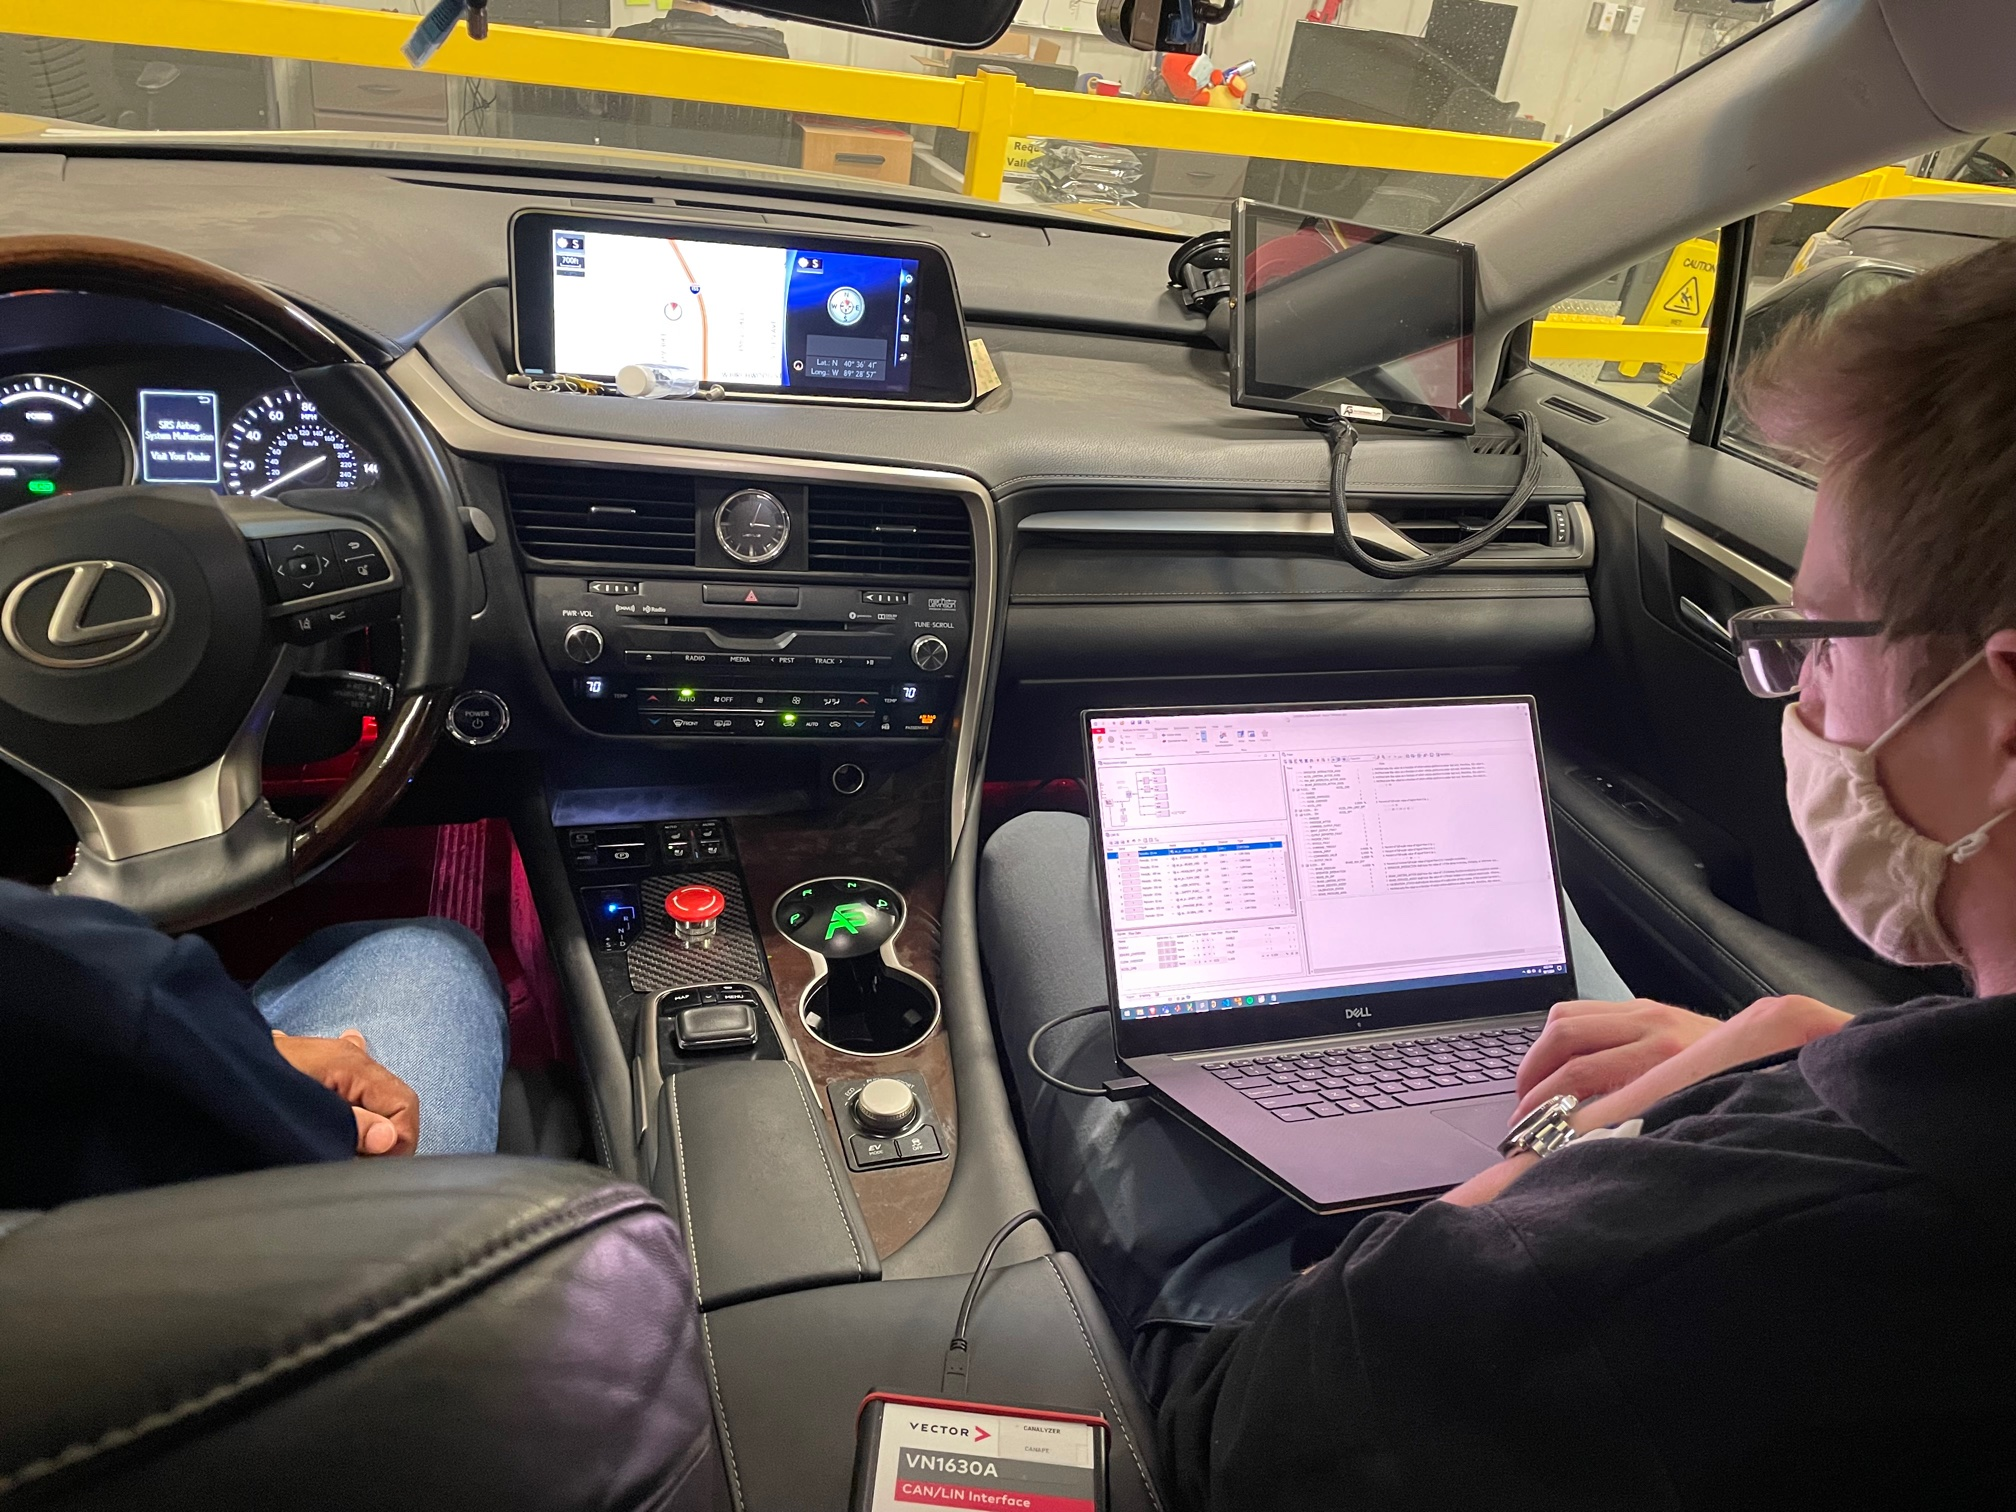
\includegraphics[width=1in]{figs/img/picturesVisitToAStuff/dataColletionSetup1-20211007}
    			\caption{Autonomous Vehicle Data Collection Setup}
    			\label{fig:vehicleSetup}
		\end{figure}
	\end{block}
\end{frame}

\begin{frame}{Validation and Testing}{Validation Setup}
	\begin{figure}
		\centering	
		\begin{minipage}{.5\textwidth}
	  		\centering
	  		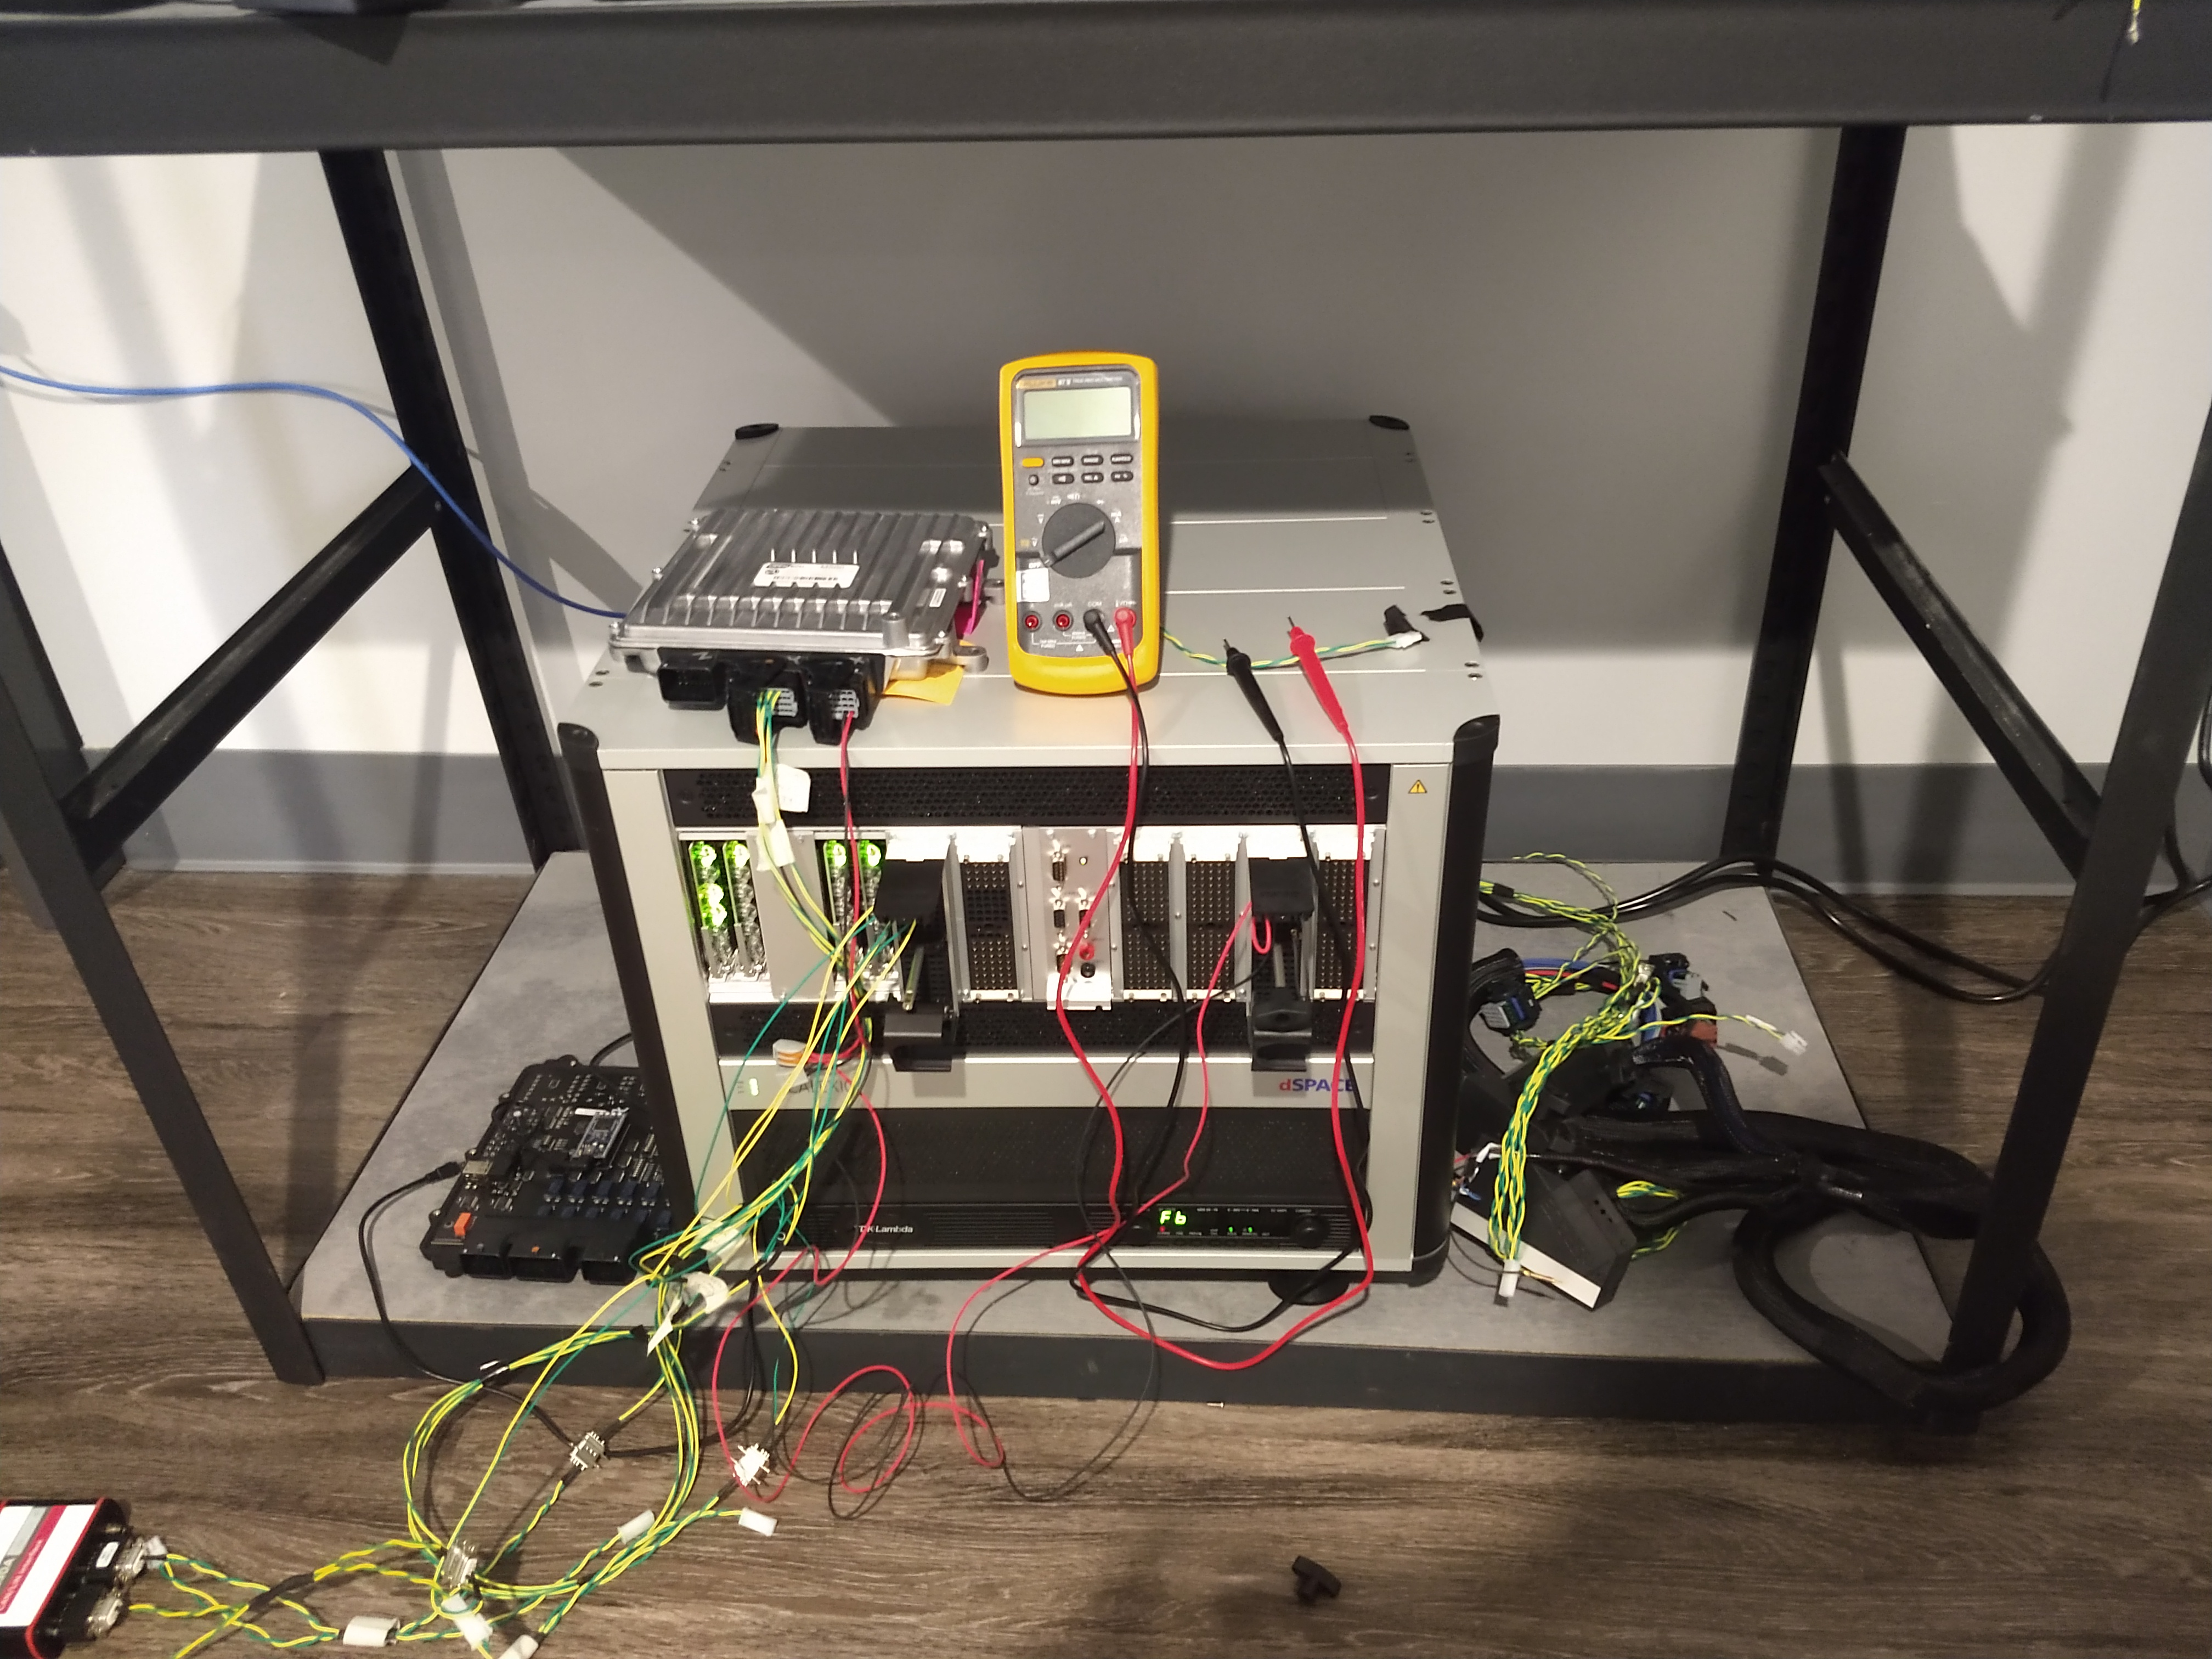
\includegraphics[width=.85\linewidth]{figs/img/picturesVisitToAStuff/hilBenchAstuff}
	  		%\captionof{figure}{A figure}
	  		\label{fig:test1}
		\end{minipage}%
		\begin{minipage}{.5\textwidth}
	  		\centering
	  		\begin{itemize} 
	  			\item HIL Bench
	  			\item Measuring output voltages to confirm results 
	  		\end{itemize}
		\end{minipage}
	\end{figure}
\end{frame}

\begin{frame}
	\begin{figure}
		\centering	
		\begin{minipage}{.5\textwidth}
	  		\centering
	  		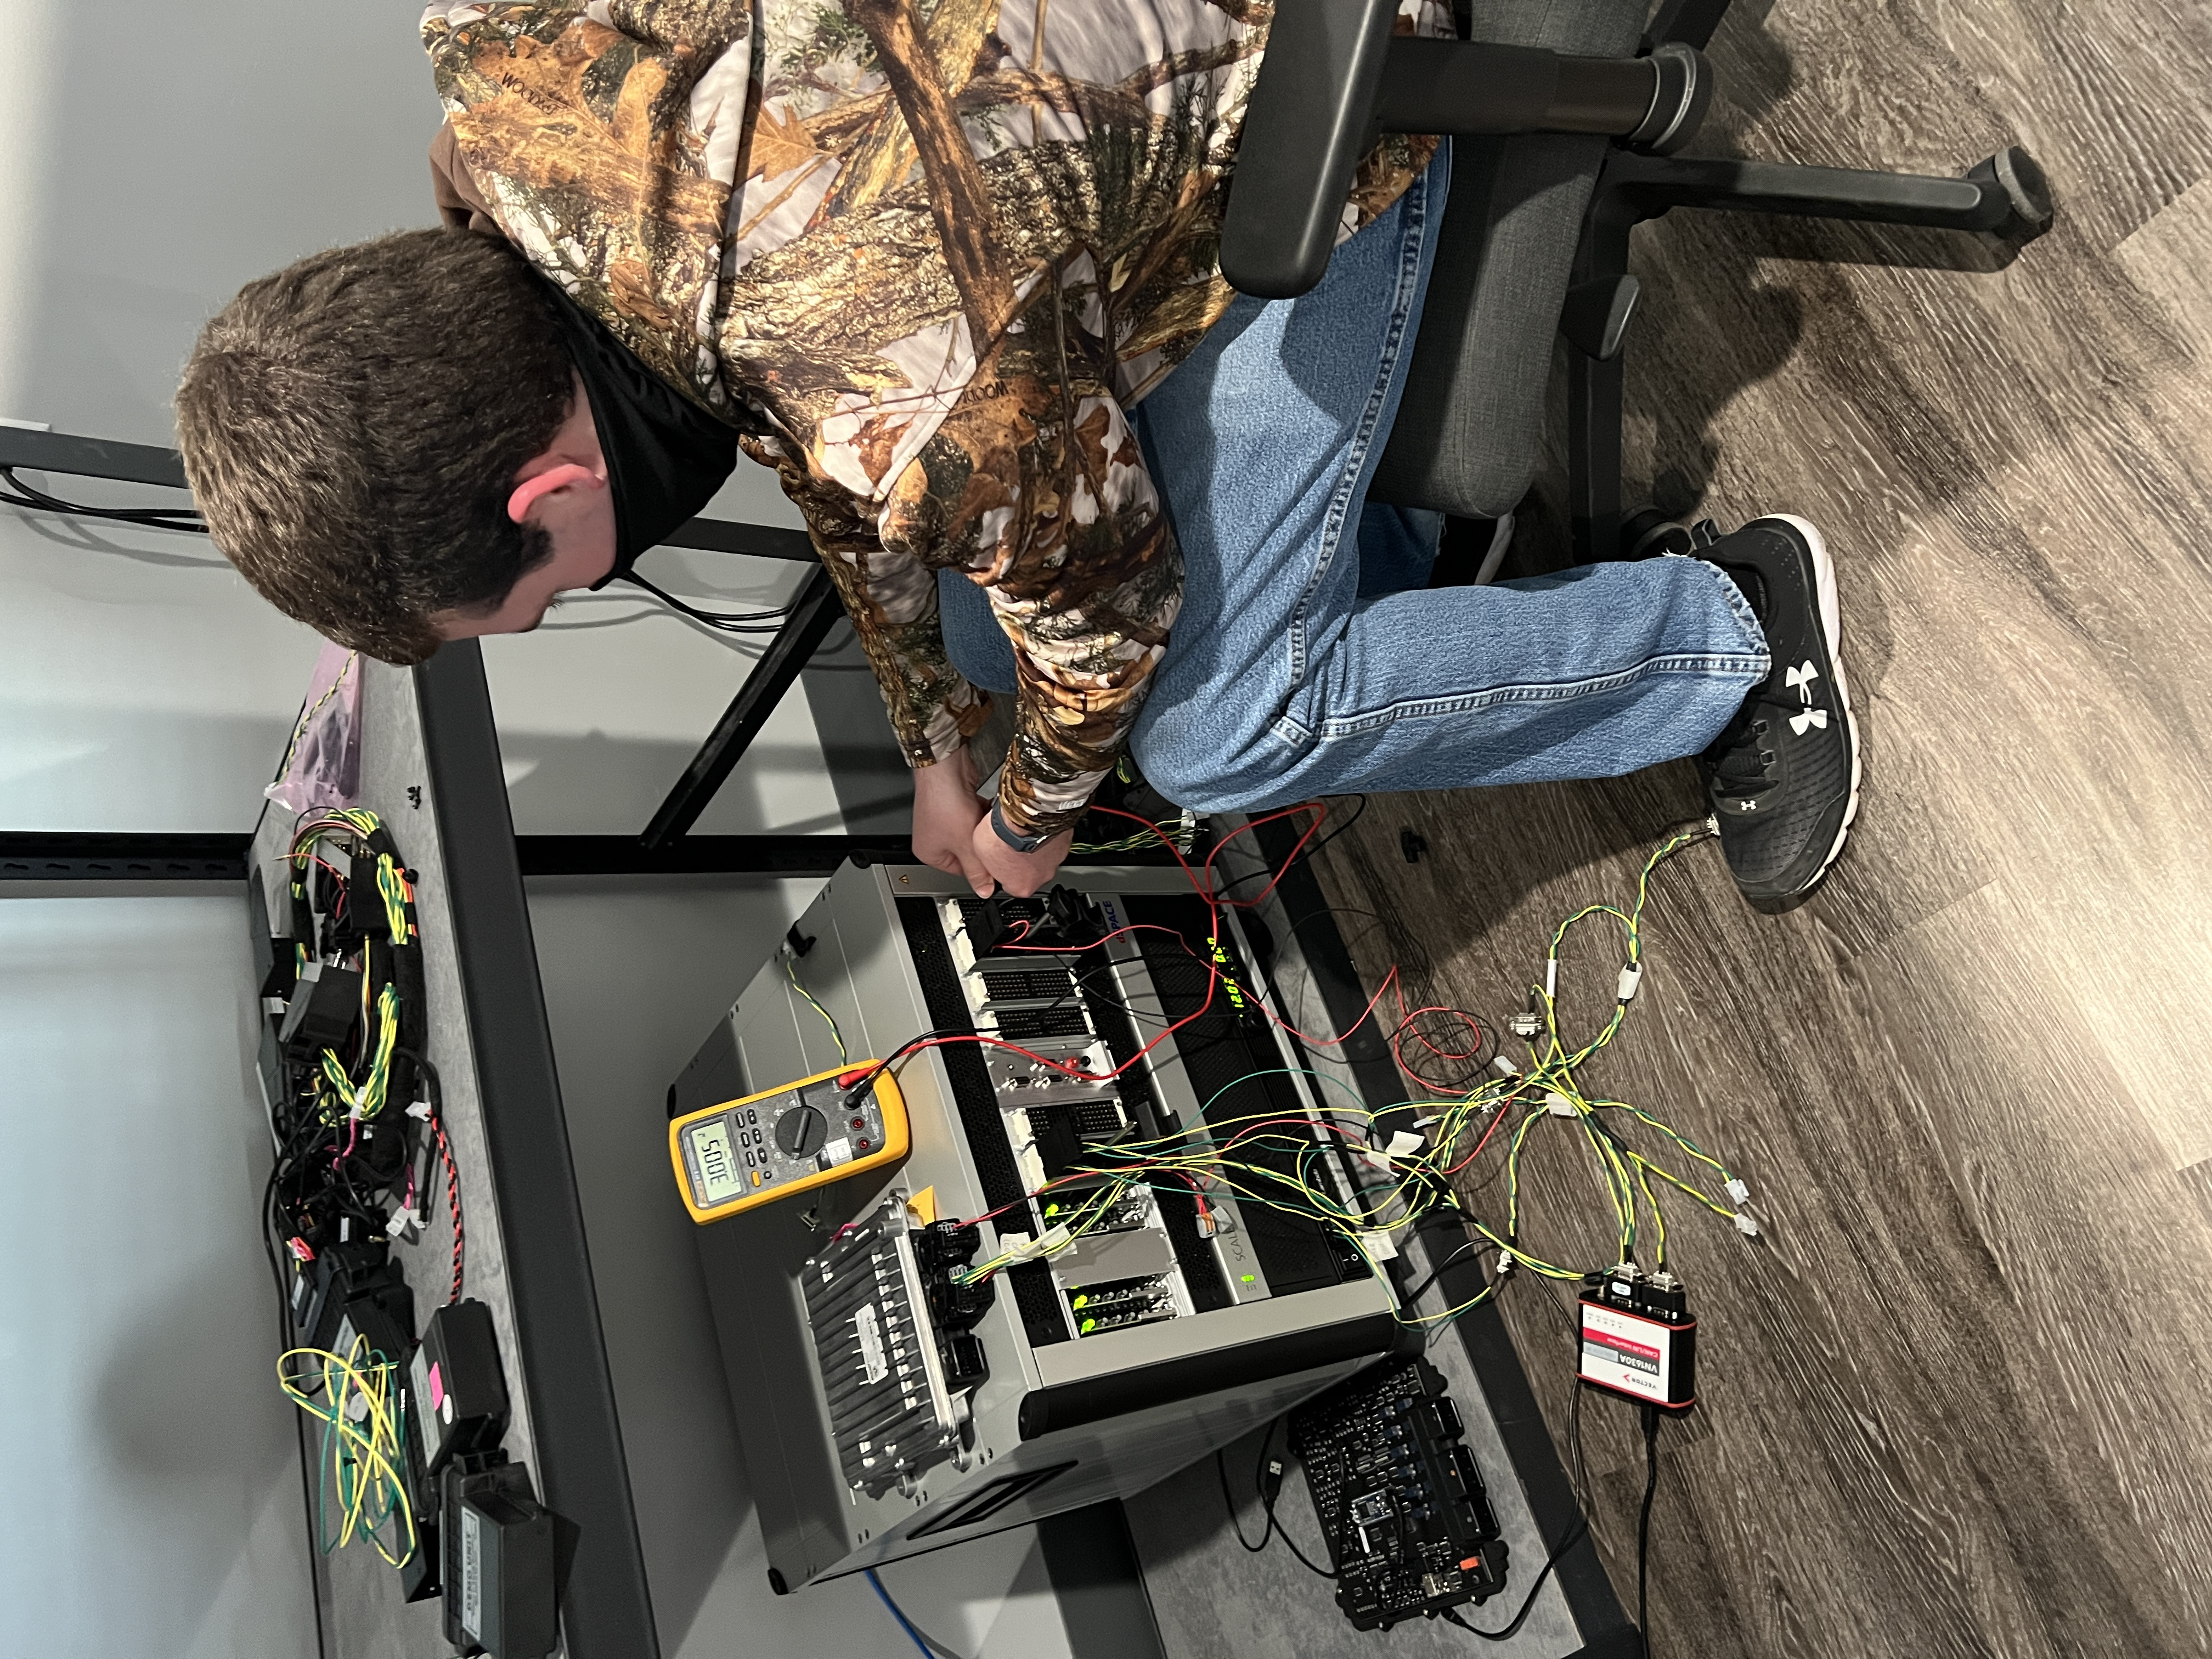
\includegraphics[angle=270,width=.85\linewidth]{figs/img/picturesVisitToAStuff/aStuffVisit2Nick}
	  		%\captionof{figure}{A figure}
	  		\label{fig:test1}
		\end{minipage}%
		\begin{minipage}{.5\textwidth}
	  		\centering
	  		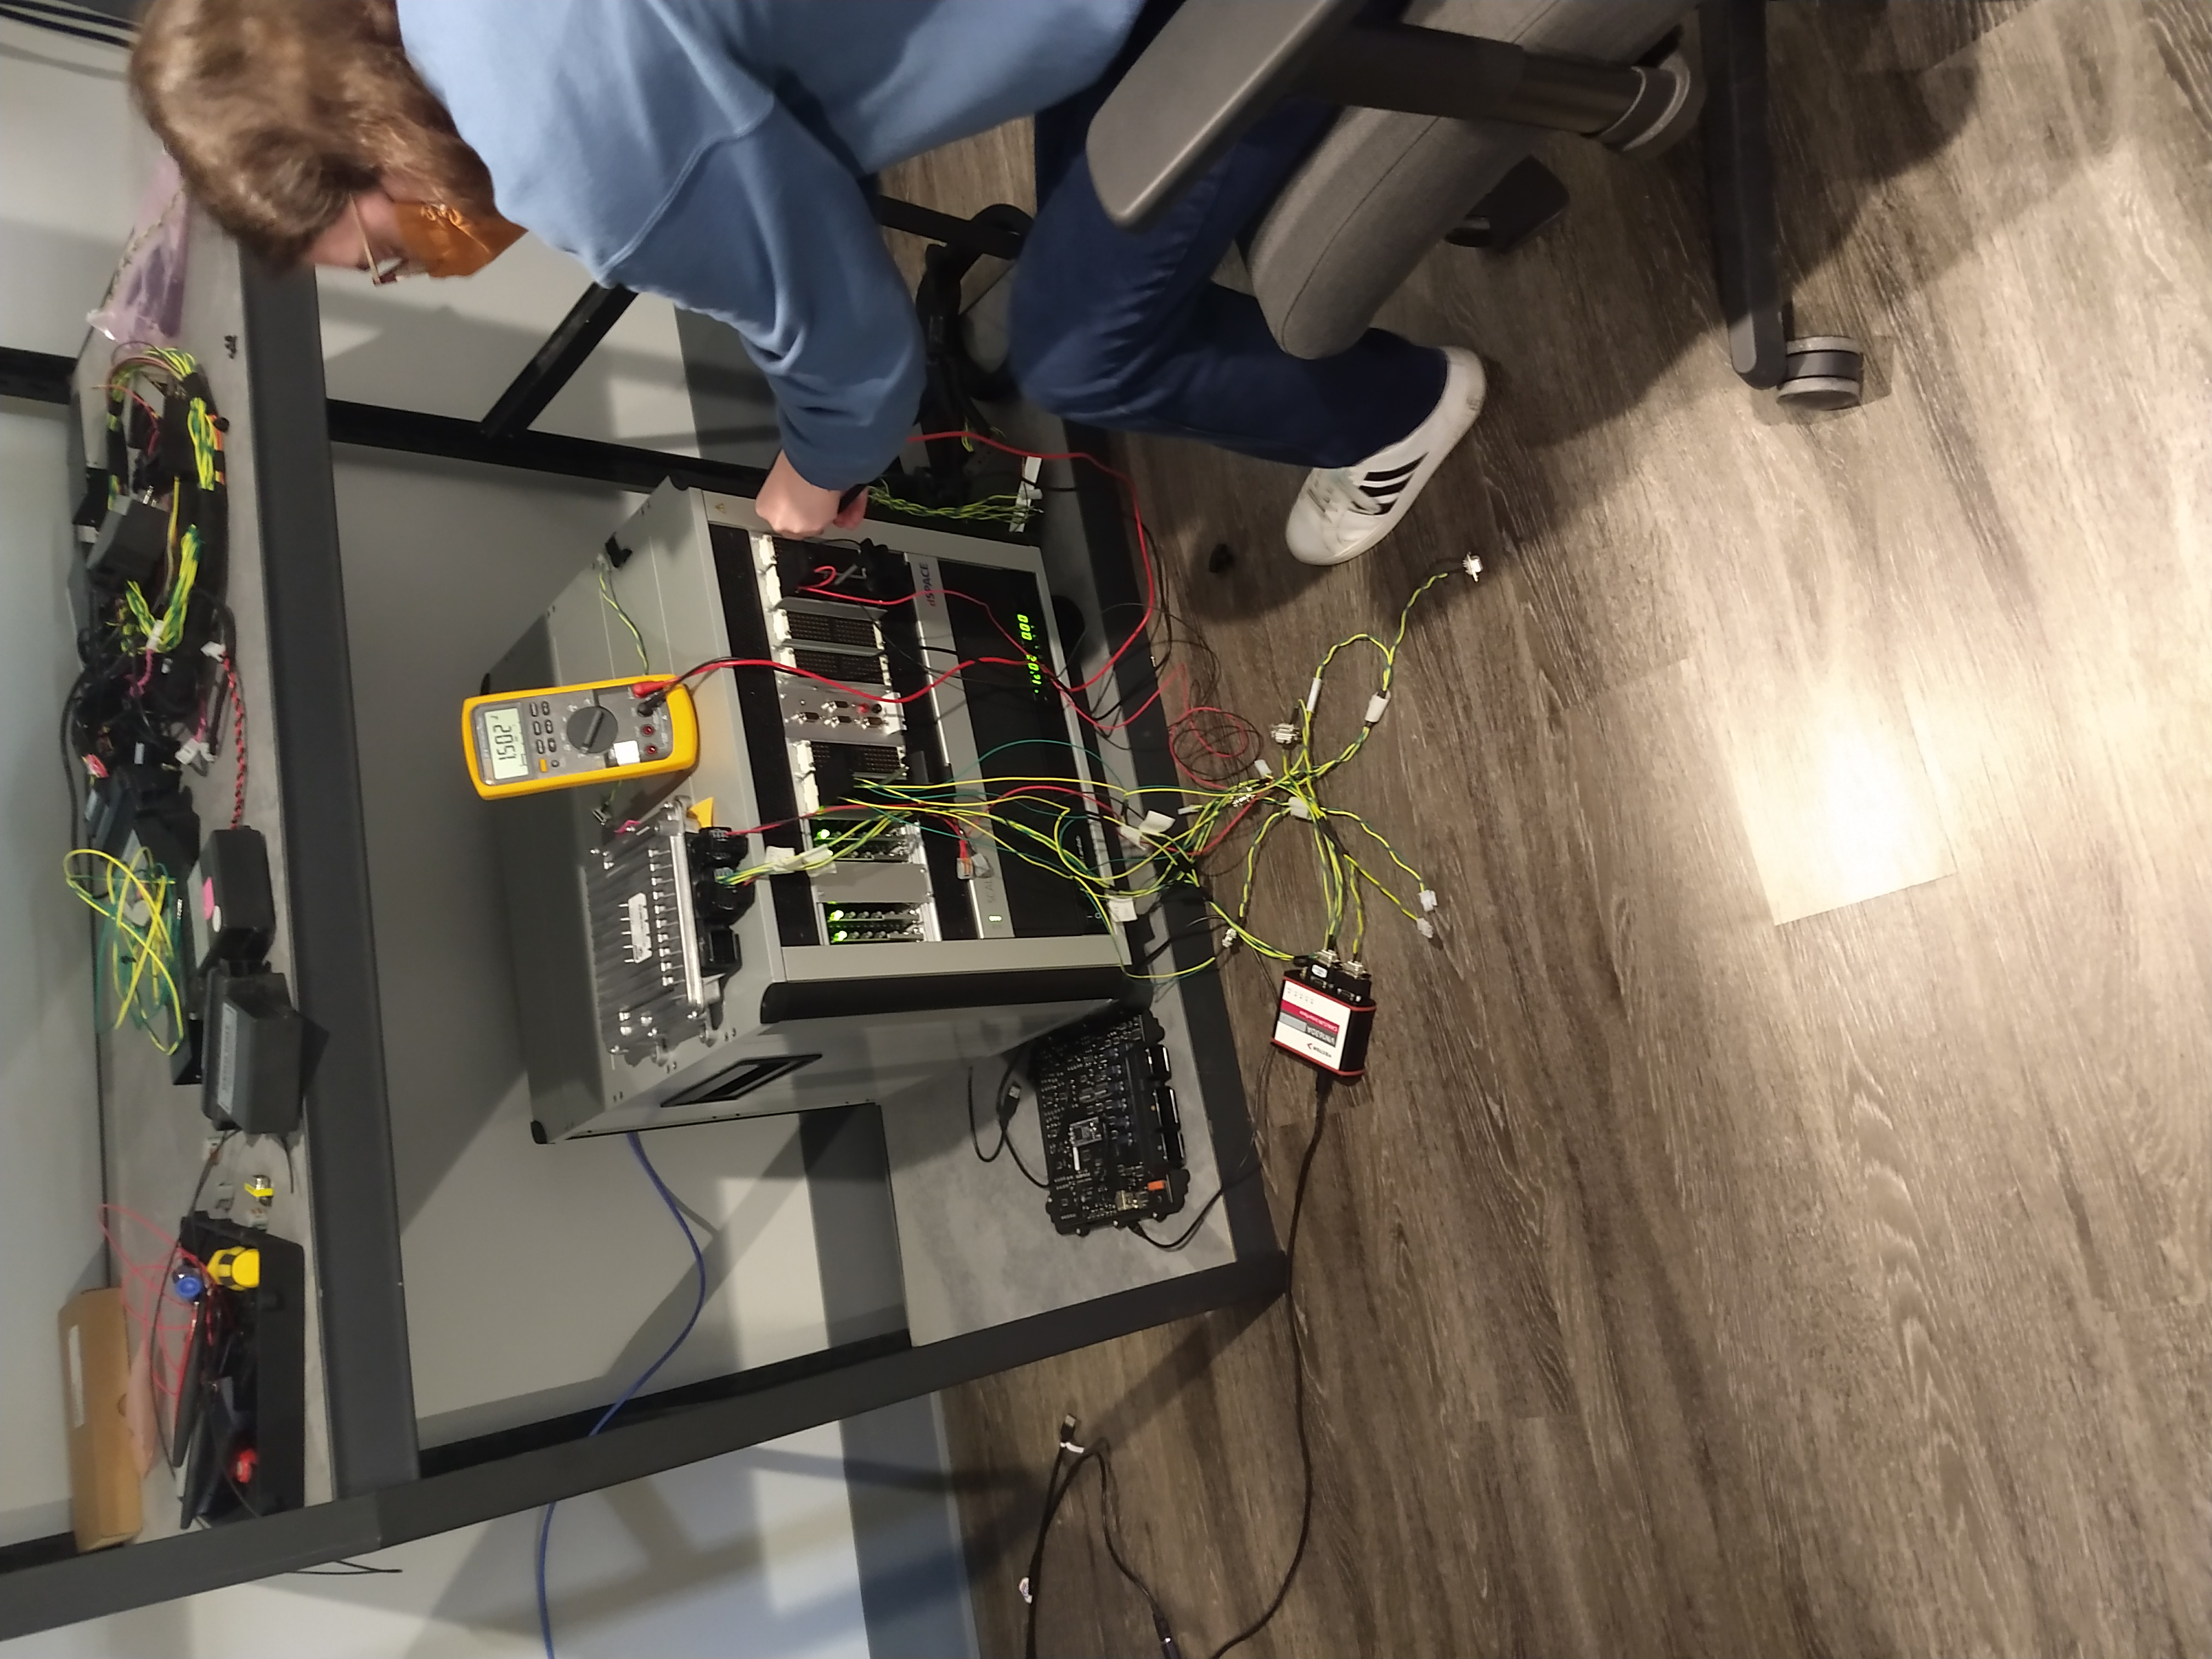
\includegraphics[angle=270,width=.85\linewidth]{figs/img/picturesVisitToAStuff/hilMeasurementHannah}
	  		%\captionof{figure}{Another figure}
	  		\label{fig:test2}
		\end{minipage}
	\end{figure}
\end{frame}

\begin{frame}{Validation and Testing}{Model Validation}
	\begin{block}{}	
		\begin{itemize}
			\item Testing data points using Control Desk software  
		\end{itemize}		
		\begin{figure}
			\centering 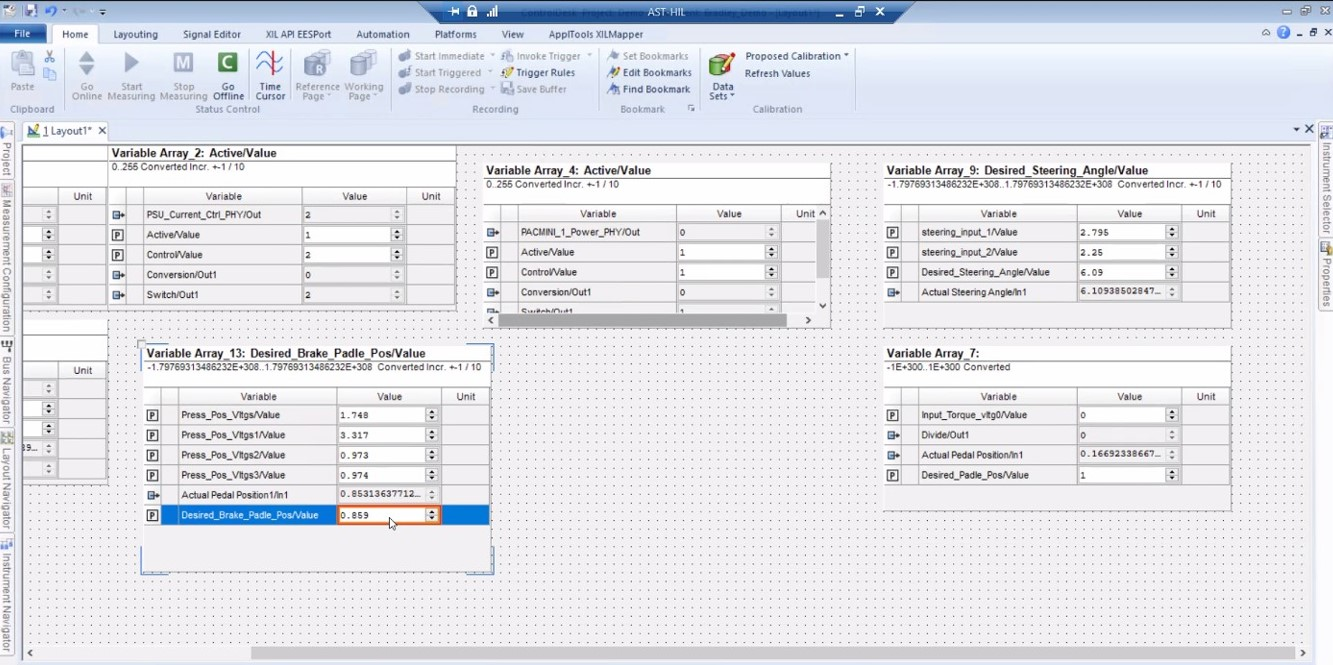
\includegraphics[width=.9\linewidth]{figs/img/aStuffValidationBrakeModel}
			\caption{Model Validation Setup}
    				\label{fig:validationSetup}
		\end{figure}
	\end{block}
\end{frame}


%------------------------------------------------------------------------------
%     SECTION BREAK
%------------------------------------------------------------------------------

\section{Conclusions and Future Work}

\begin{frame}{Conclusions and Future Work}
  \begin{block}{Conclusions and Challenges}
    \begin{itemize}
      \item Conclusions
      \begin{itemize}
      	\item Switch from transfer function to neural network models
      	\item Neural network modeling worked best 
      \end{itemize}
      \item Challenges
        \begin{itemize}
      	\item Time constraints 
      	\item Hardware constraints 
      \end{itemize}
    \end{itemize}
  \end{block}
  \begin{block}{Future Work}
    \begin{itemize}
    	  \item Model shift, speed, and speed control subsystems
      \item Test models using Hardware-in-the-Loop
      \item Create new vehicle controllers 
    \end{itemize}
  \end{block}
\end{frame}

%------------------------------------------------------------------------------
%     SECTION BREAK
%------------------------------------------------------------------------------

\section{References}

\begin{frame}[allowframebreaks]{References}
  \bibliographystyle{IEEEtran}
  \bibliography{bib/references.bib}
\end{frame}

%==============================================================================
%==============================================================================
%     END OF SLIDES
%==============================================================================
%==============================================================================

\end{document}

%%% Local Variables:
%%% mode: latex
%%% TeX-master: t
%%% End:
